\documentclass[a4paper,12pt]{article}

\usepackage{graphicx} % Required for inserting images
\usepackage{amsmath,amssymb,amsfonts}
\usepackage{subcaption}
% -----------------------
% Package Imports
% -----------------------

% Set page margins
\usepackage[a4paper, top=1in, bottom=0.8in, left=1.1in, right=0.8in]{geometry}

% Use Times New Roman font
\usepackage{times}

% Add page numbering
\pagestyle{plain}
\usepackage{multirow}
% Enable graphics inclusion
\usepackage{graphicx}
\usepackage{float}
% Enable code listings
\usepackage{listings}
\usepackage{xcolor} % For customizing code colors

% Define MATLAB style for listings
\lstdefinestyle{vscode-light}{
	language=Matlab,
	basicstyle=\ttfamily\footnotesize,
	keywordstyle=\color{black},
	commentstyle=\color{gray},
	stringstyle=\color{red},
	numberstyle=\tiny\color{black},
	numbersep=5pt,
	frame=single,
	backgroundcolor=\color{white!10},
	breaklines=true,
	captionpos=b,
	tabsize=4,
	showstringspaces=false,
	numbers=left,  % Enable line numbering on the left
	stepnumber=1,  % Line numbers increment by 1
	numberfirstline=true, % Number the first line
}
\setlength{\parindent}{0pt}
\usepackage{titlesec} % To customize section font size
\titleformat{\section}
{\normalfont\fontsize{14}{16}\bfseries}{\thesection}{1em}{}

\titleformat{\subsection}
{\normalfont\fontsize{14}{16}\bfseries}{\thesubsection}{1em}{}


\begin{document}
	\section{Experiment No. 4}
	
	\section{Experiment Title }
	Observation \& Verification of fault analysis for color TV (Cathode Ray \& LED TV) .
	\section{Objective}
	
	
	
	The objectives of this lab are as follows:
	\begin{itemize}
		\item To analyze the system's response to these faults.
		\item To demonstrate and understand different types of faults.
	
	\end{itemize}
	
	\section{Theory}
	
	
	
	Fault switches are there to make user understand the effect of the particular switch. Fault Switch schemes are protection functions intended to trip a transmission line breaker when closed on to a faulted line. Dedicated fault switches are available in various designs, but since the fault-detecting elements tend to be more sensitive than conventional, impedance-based line protection functions, they are generally designed to be "armed" only for a brief period following breaker closure. Depending on the details of scheme design and element settings, there may be implications for line relay loadability.
	\subsection{GENERAL CHARACTERISTICS OF THE TRAINER DL 2402}
	
	
	The trainer is composed of modular elements assembled in the metallic frame containing the front panel of the trainer itself.
	
	The trainer front panel includes the synoptic panel that reproduces the diagram of the equipment in a simplified form, suitable to the educational use and to the collective carrying out of the exercises.
	
	The measurement points of the front panel are composed of 2 mm terminals to which it is possible to connect both external instruments and equipments.
	
	It is important that the measurement points are not short-circuited among them or towards ground. This could cause bad operations in the equipment, even if in the equipment suitable protections have been included.

	
		\begin{figure}[H]
		\centering
		\begin{subfigure}[t]{0.49\textwidth}
			\centering
			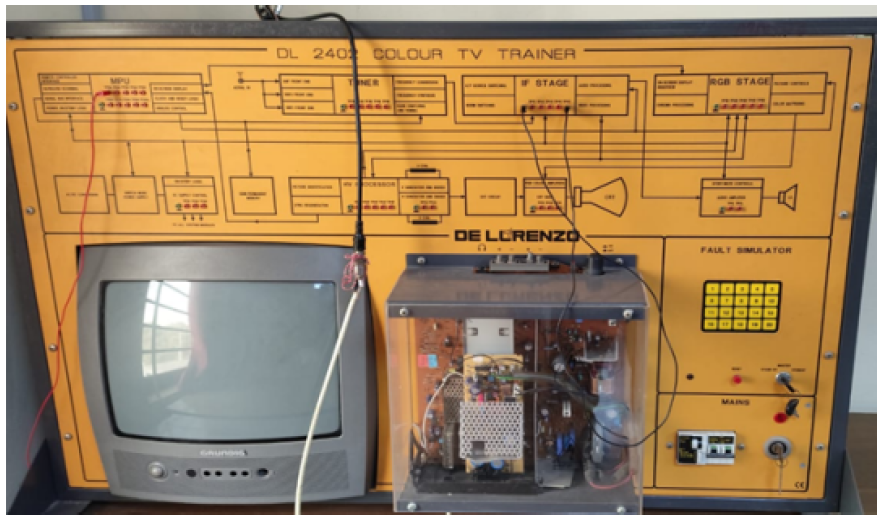
\includegraphics[width=1\linewidth, height=0.205\textheight]{Images/2}
			\caption{DL 2402 Colour TV Trainer}
			\vspace{0.1cm}
		\end{subfigure}
	\end{figure}
		The functional study of the TVC can be carried out with the only access of test-points of the synoptic panel. In-depth study of the trainer requires the removal of the protective transparent cover. The electronic boards become therefore accessible.
	Since potentially hazardous voltages become accessible, it is recommended in this case that the students are duly instructed on general and specific safety rules.
	
	On the front panel the fault simulator is assembled, that can be either with microprocessor (DL 2402M) or with microswitch (DL 2402A or DL 2402K).
	
	This manual is valid for both the versions, both for what is referred to the description of the equipments and to the exercises. Some sections, however, can be used by one of the two versions and this is clearly specified in the title or in the relative paragraphs.
	
	
	
	\section{Required Apparatus}
	\begin{enumerate}
		
		\item 	DL 2402 Colour TV Trainer.
		\item   LCD/LED TV Trainer ( KVT-05A/B Trainer Kit).
		\item	Oscilloscope (TBS-1000c).
		\item  Connecting wires \& Probes.
	\end{enumerate}
	\section{Experimental Setup}
	\begin{figure}[H]
		\centering
		\begin{subfigure}[t]{0.49\textwidth}
			\centering
			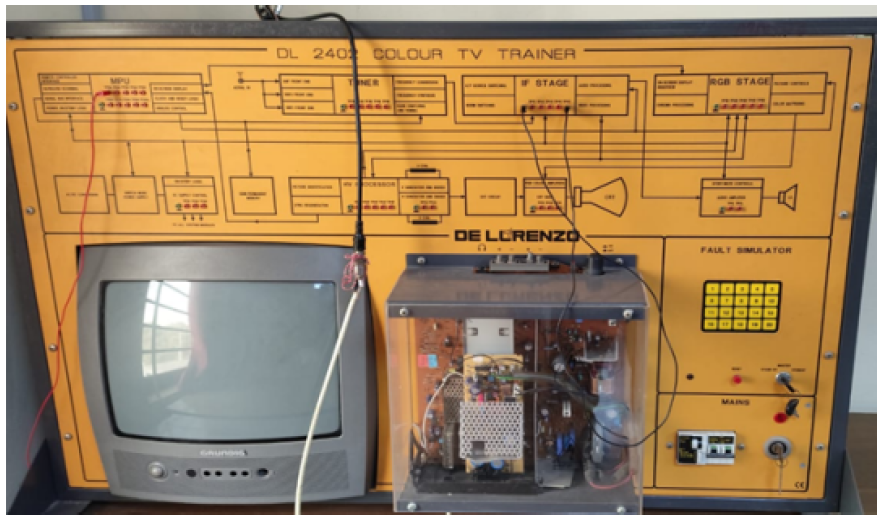
\includegraphics[width=1\linewidth, height=0.205\textheight]{Images/2}
			\caption{DL 2402 Colour TV Trainer}
			\vspace{0.1cm}
		\end{subfigure}
		\hfil
		\begin{subfigure}[t]{0.49\textwidth}
			\centering
			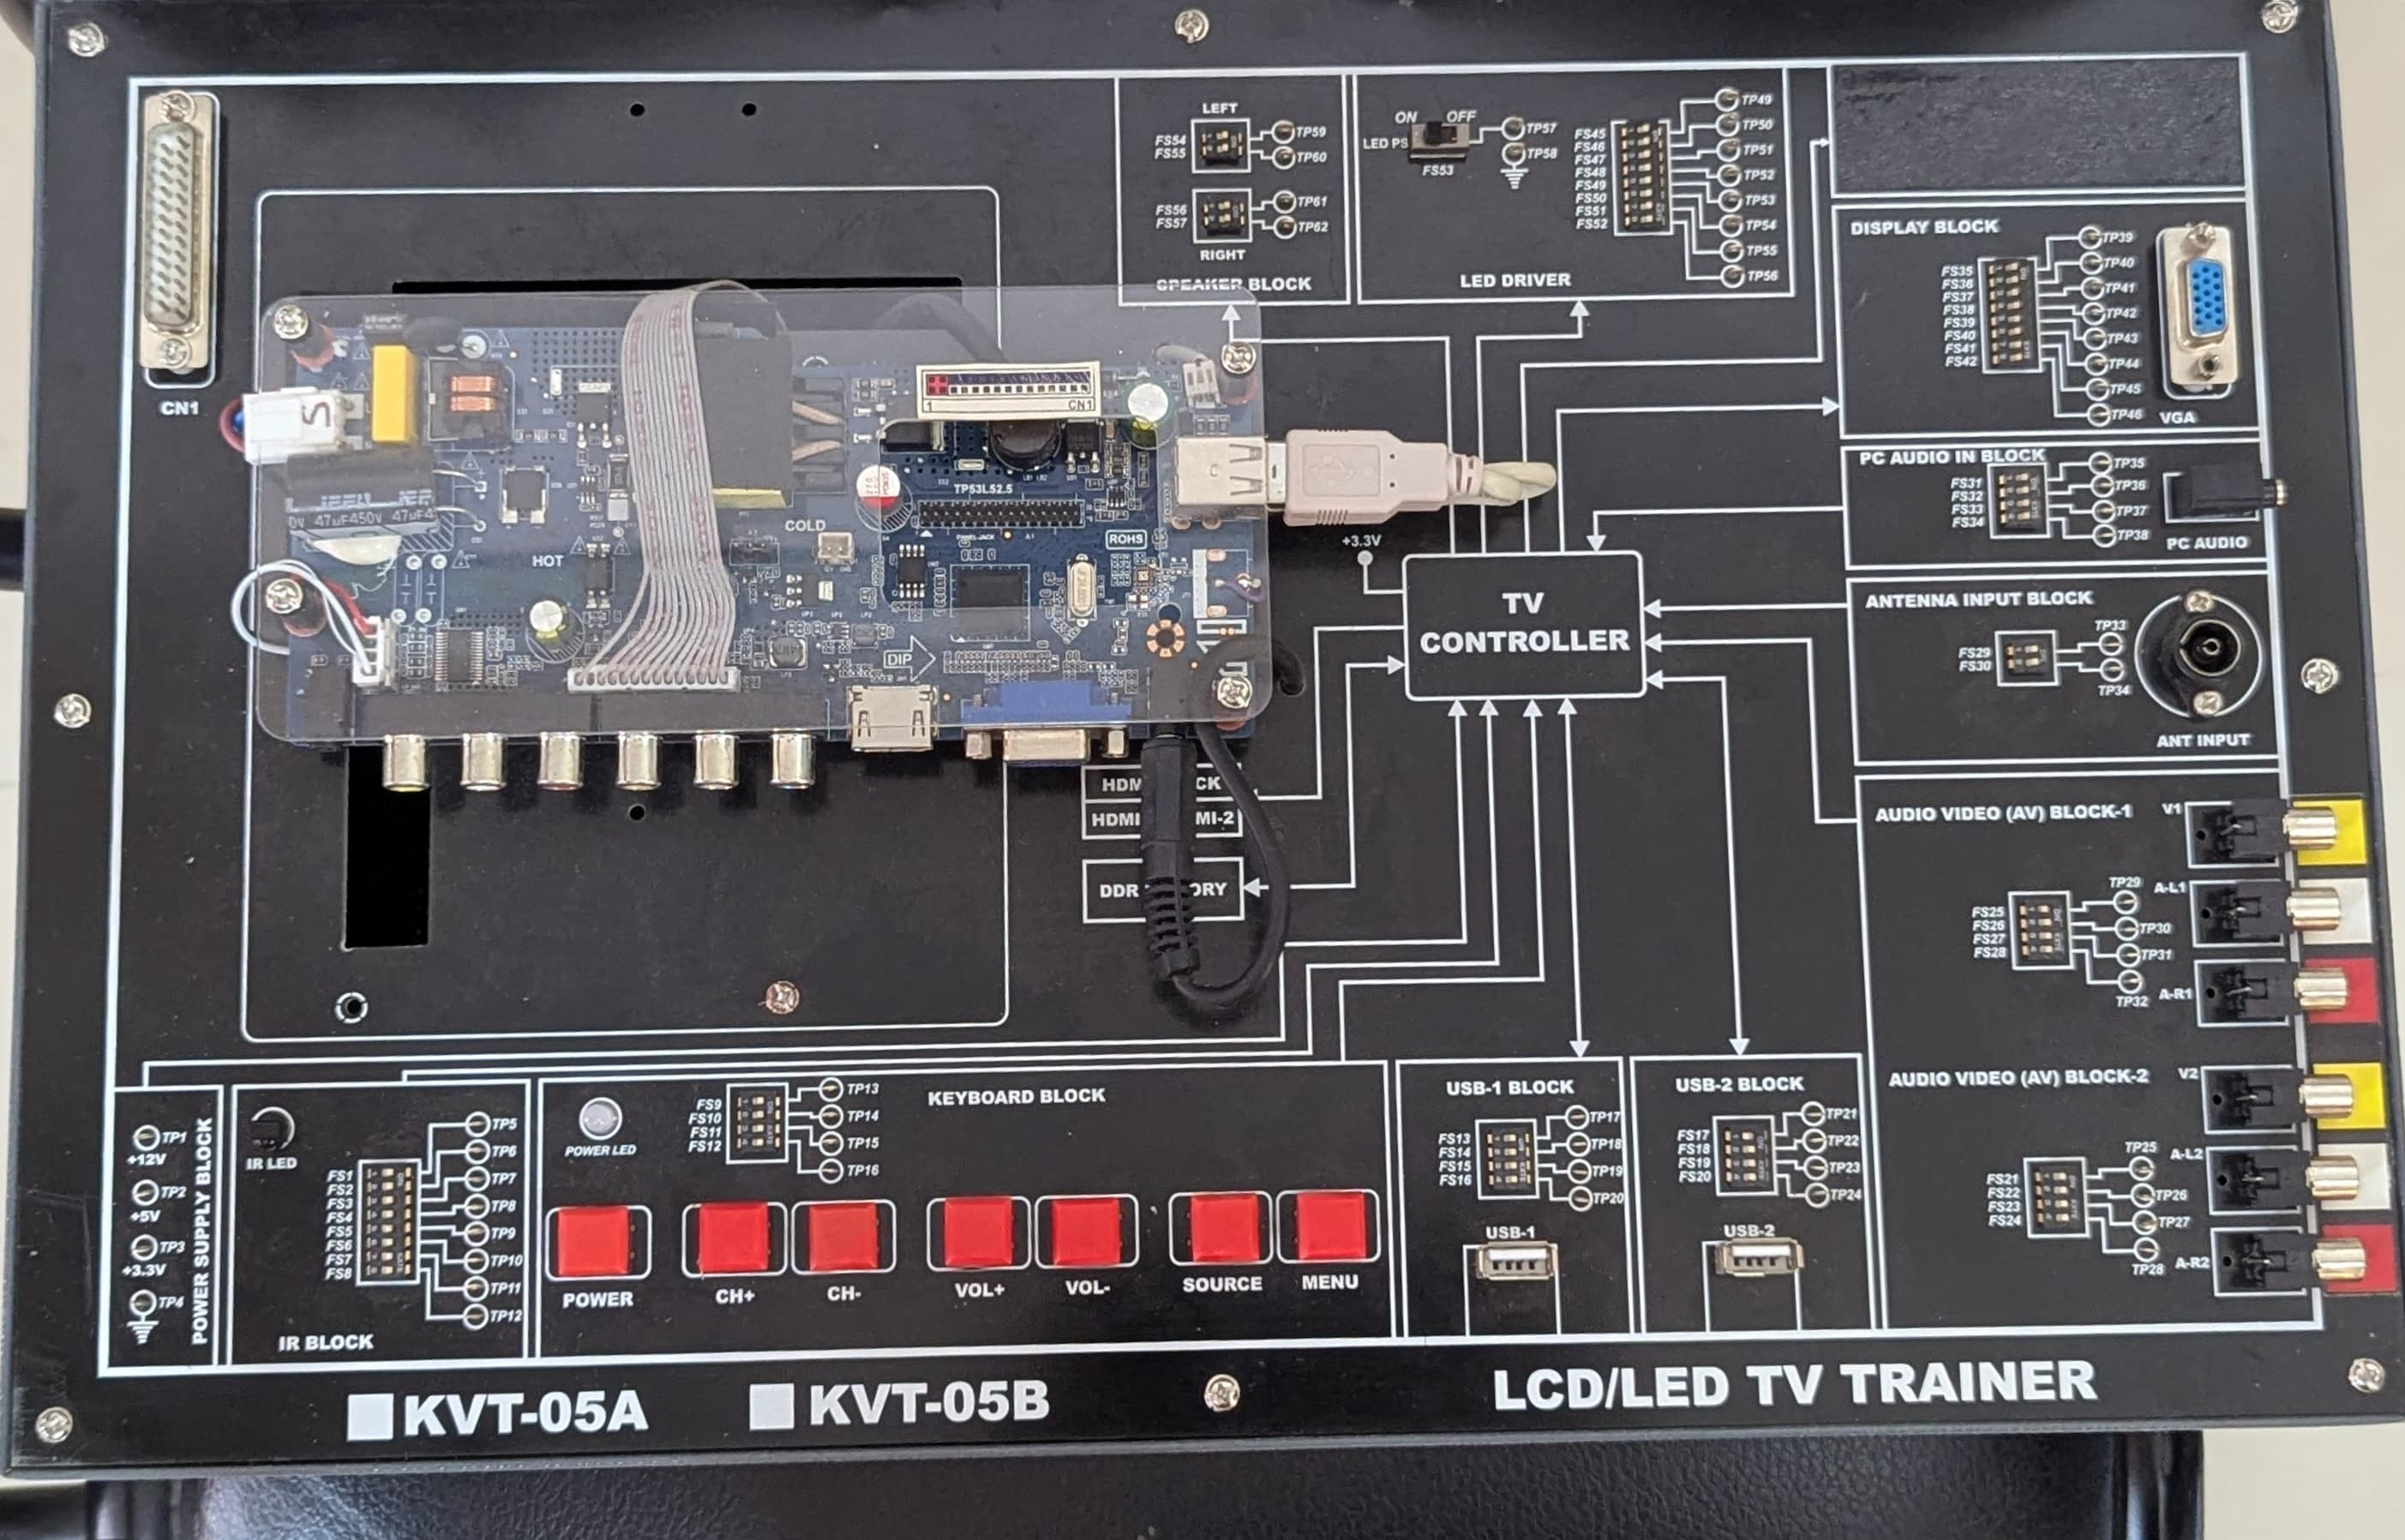
\includegraphics[width=1\linewidth]{Images/1}
			\caption{KVT-05A/B LED TV TrainerTrainer Kit}
		\end{subfigure}
	\end{figure}
	
	\section{Procedure for LED TV fault analysis}
\begin{enumerate}
	\item Connect AC Supply to the kit.
	\item Press "POWER" switch.
	\item Keep all the fault switches FS1-FS57 at ON Position.
	\item Make the switch faults as given in the following table and observe the result.
\end{enumerate}
\newpage
	\subsection{Locations \& Observations of faults for LED TV}
	
\begin{table}[H]
	\centering
	\caption{FS1-FS8 (IR and Keyboard Block)}
\begin{tabular}{|c|c|l|}
	
	\hline
	\textbf{Faults No} & \textbf{DIP Switch} & \multicolumn{1}{c|}{\textbf{ Observations (Switch is off) }} \\
	\hline
	1 & Pin-1 & Remote control will not work \\
	\hline
	2 & Pin-2 & Power key will not work \\
	\hline
	3 & Pin-3 & CH+ key will not work \\
	\hline
	4 & Pin-4 & CH- key will not work \\
	\hline
	5 & Pin-5 & V+ key will not work \\
	\hline
	6 & Pin-6 & V- key will not work \\
	\hline
	7 & Pin-7 & Menu key will not work \\
	\hline
	8 & Pin-8 & Source key will not work \\
	\hline
\end{tabular}
\end{table}

	\begin{table}[H]
		
		\centering
		\caption{FS21-FS24 (Audio Video Block-2)}
		\begin{tabular}{|c|c|l|}
			\hline
			\textbf{Sr. No} & \textbf{DIP Switch} & \multicolumn{1}{c|}{\textbf{Observations (Switch is off)}} \\
			\hline
			1 & Pin-1 & Video Signal  got cut off, hence No Video/Audio \\
			\hline
			2 & Pin-2 & Left Audio didn't not work \\
			\hline
			3 & Pin-3 & Right Audio didn't not work \\
			\hline
			4 & Pin-4 & All Switches Common GND, No Audio/Video \\
			\hline
		\end{tabular}
		
	\end{table}
	
		
	\begin{table}[H]
	\centering
	\caption{FS25-FS28 (Audio Video Block-2)}
	\begin{tabular}{|c|c|l|}
		\hline
		\textbf{Sr. No} & \textbf{DIP Switch} & \multicolumn{1}{c|}{\textbf{Observations (Switch is off)}} \\
		\hline
		1 & Pin-1 & Video Signal got cut off, hence No Video/Audio \\
		\hline
		2 & Pin-2 & Left Audio didn't not work \\
		\hline
		3 & Pin-3 & Right Audio didn't not work \\
		\hline
		4 & Pin-4 & All Switches Common GND, No Audio/Video \\
		\hline
	\end{tabular}
	
	\end{table}

\begin{table}[H]

\centering
\caption{FS35-FS42 (Display Block)}
\begin{tabular}{|c|c|l|}
	\hline
	\textbf{Sr. No} & \textbf{DIP Switch} & \multicolumn{1}{c|}{\textbf{Observations (Switch is off)}} \\
	\hline
	1 & Pin-1 & RED Colour got eliminated from the image \\
	\hline
	2 & Pin-2 & GREEN Colour got eliminated from the image \\
	\hline
	3 & Pin-3 & BLUE Colour got eliminated from the image \\
	\hline
	4 & Pin-4 & HORIZONTAL SYNC was missing, hence monitor gets Blank \\
	\hline
	5 & Pin-5 & VERTICAL SYNC was missing, hence monitor got Blank \\
	\hline
	6,7 \& 8 & Pin-6,7 \& 8 & GND  got disconnected, no display. \\
	\hline
\end{tabular}

\end{table}
	
	
\newpage
\section{Procedure for Cathode-ray TV fault analysis}
\begin{enumerate}
	\item Connect AC Supply to the kit.
	\item Press "POWER" switch.
	\item Keep the fault switches ON Position once at a time.
	\item Make the switch faults as given in the following table and observe the result.
\end{enumerate}
\subsection{Locations \& Observations of faults for Cathode-ray TV}
\begin{table}[H]
	\centering
	\caption{Fault analysis of Cathode-ray TV}
	\begin{tabular}{|c|c|c|c|}
		\hline
		\textbf{Fault Number} & \textbf{Location}                                                   & \textbf{Observation}                                                                                       & \textbf{\begin{tabular}[c]{@{}c@{}}Oscilloscope \\ Observation\end{tabular}} \\ \hline
		1                     & Remote  control                                                     & No fault detected                                                                                          & Straight line                                                                \\ \hline
		2                     & \begin{tabular}[c]{@{}c@{}}Key-board\\  operation\end{tabular}      & No fault detected                                                                                          & \begin{tabular}[c]{@{}c@{}}Distorted\\ spikey wave\end{tabular}              \\ \hline
		3                     & \begin{tabular}[c]{@{}c@{}}Reset of\\  microcontroller\end{tabular} & Power off                                                                                                  & Straight line                                                                \\ \hline
		4                     & Audio                                                               & Only audio,no video                                                                                        & Straight line                                                                \\ \hline
		5                     & \begin{tabular}[c]{@{}c@{}}On-screen-\\ display\end{tabular}        & Display flickered                                                                                          & \begin{tabular}[c]{@{}c@{}}Chain shaped\\  wave\end{tabular}                 \\ \hline
		6                     & \begin{tabular}[c]{@{}c@{}}On-screen-\\ display\end{tabular}        & Sound flickered                                                                                            & Straight line                                                                \\ \hline
		7                     & \begin{tabular}[c]{@{}c@{}}On-screen-\\ display\end{tabular}        & Sound flickered                                                                                            & Straight line                                                                \\ \hline
		8                     & RGB stage                                                           & Sound flickered                                                                                            & Spike                                                                        \\ \hline
		9                     & \begin{tabular}[c]{@{}c@{}}On-screen\\ -display\end{tabular}        & \begin{tabular}[c]{@{}c@{}}Sound flickered, \\  faded display\end{tabular}                                 & \begin{tabular}[c]{@{}c@{}}Two parallel\\  straight line\end{tabular}        \\ \hline
		10                    & \begin{tabular}[c]{@{}c@{}}On-screen-\\ display\end{tabular}        & Audio on, display off                                                                                      & Straight line                                                                \\ \hline
		11                    & Tuner                                                               & Audio off, display on                                                                                      & Straight line                                                                \\ \hline
		12                    & Tuner                                                               & No fault detected                                                                                          & Dot signal                                                                   \\ \hline
		13                    & Tuner                                                               & No fault detected                                                                                          & Dot signal                                                                   \\ \hline
		14                    & CPU                                                                 & Yellowish display                                                                                          & Straight line                                                                \\ \hline
		15                    & IF stage                                                            & \begin{tabular}[c]{@{}c@{}}Audio off,\\  display flickered\end{tabular}                                    & Straight line                                                                \\ \hline
		16                    & IF stage                                                            & No fault detected                                                                                          & Distorted signal                                                             \\ \hline
		17                    & IF stage                                                            & \begin{tabular}[c]{@{}c@{}}Audio off,\\  greyish display\end{tabular}                                      & Blurry wave                                                                  \\ \hline
		18                    & RGB stage                                                           & Pale display                                                                                               & Spiky blur signal                                                            \\ \hline
		19                    & \begin{tabular}[c]{@{}c@{}}Picture \\ control\end{tabular}          & \begin{tabular}[c]{@{}c@{}}Black and\\  white display\end{tabular}                                         & Distorted sine wave                                                          \\ \hline
		20                    & \begin{tabular}[c]{@{}c@{}}Audio\\  amplifier\end{tabular}          & \begin{tabular}[c]{@{}c@{}}White straight line\\  in the middle of  \\  the display, audio on\end{tabular} & Blurry sine wave                                                             \\ \hline
	\end{tabular}
\end{table}
\newpage
	
\section{Fault analysis wavehape of Cathode ray TV}
\begin{figure}[H]
	\centering
	\begin{subfigure}[t]{0.44\textwidth}
		\centering
		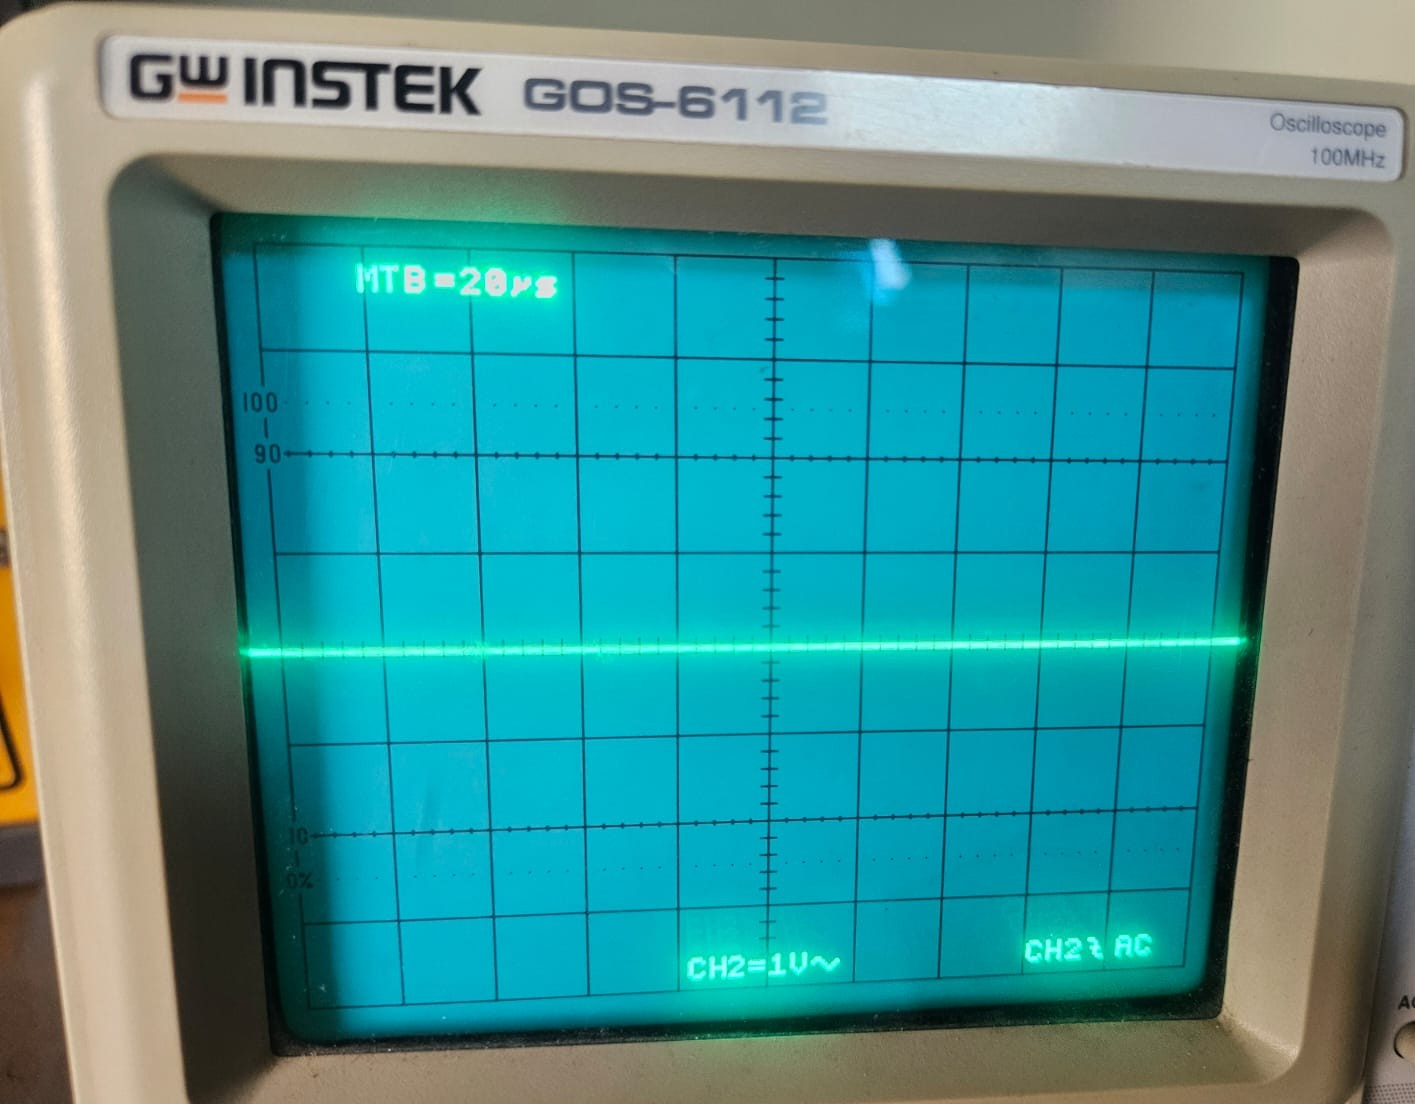
\includegraphics[width=1\linewidth]{Images/1.1}
		\caption{Fault 1}
		\vspace{0.1cm}
	\end{subfigure}
	\hfil
	\begin{subfigure}[t]{0.44\textwidth}
		\centering
		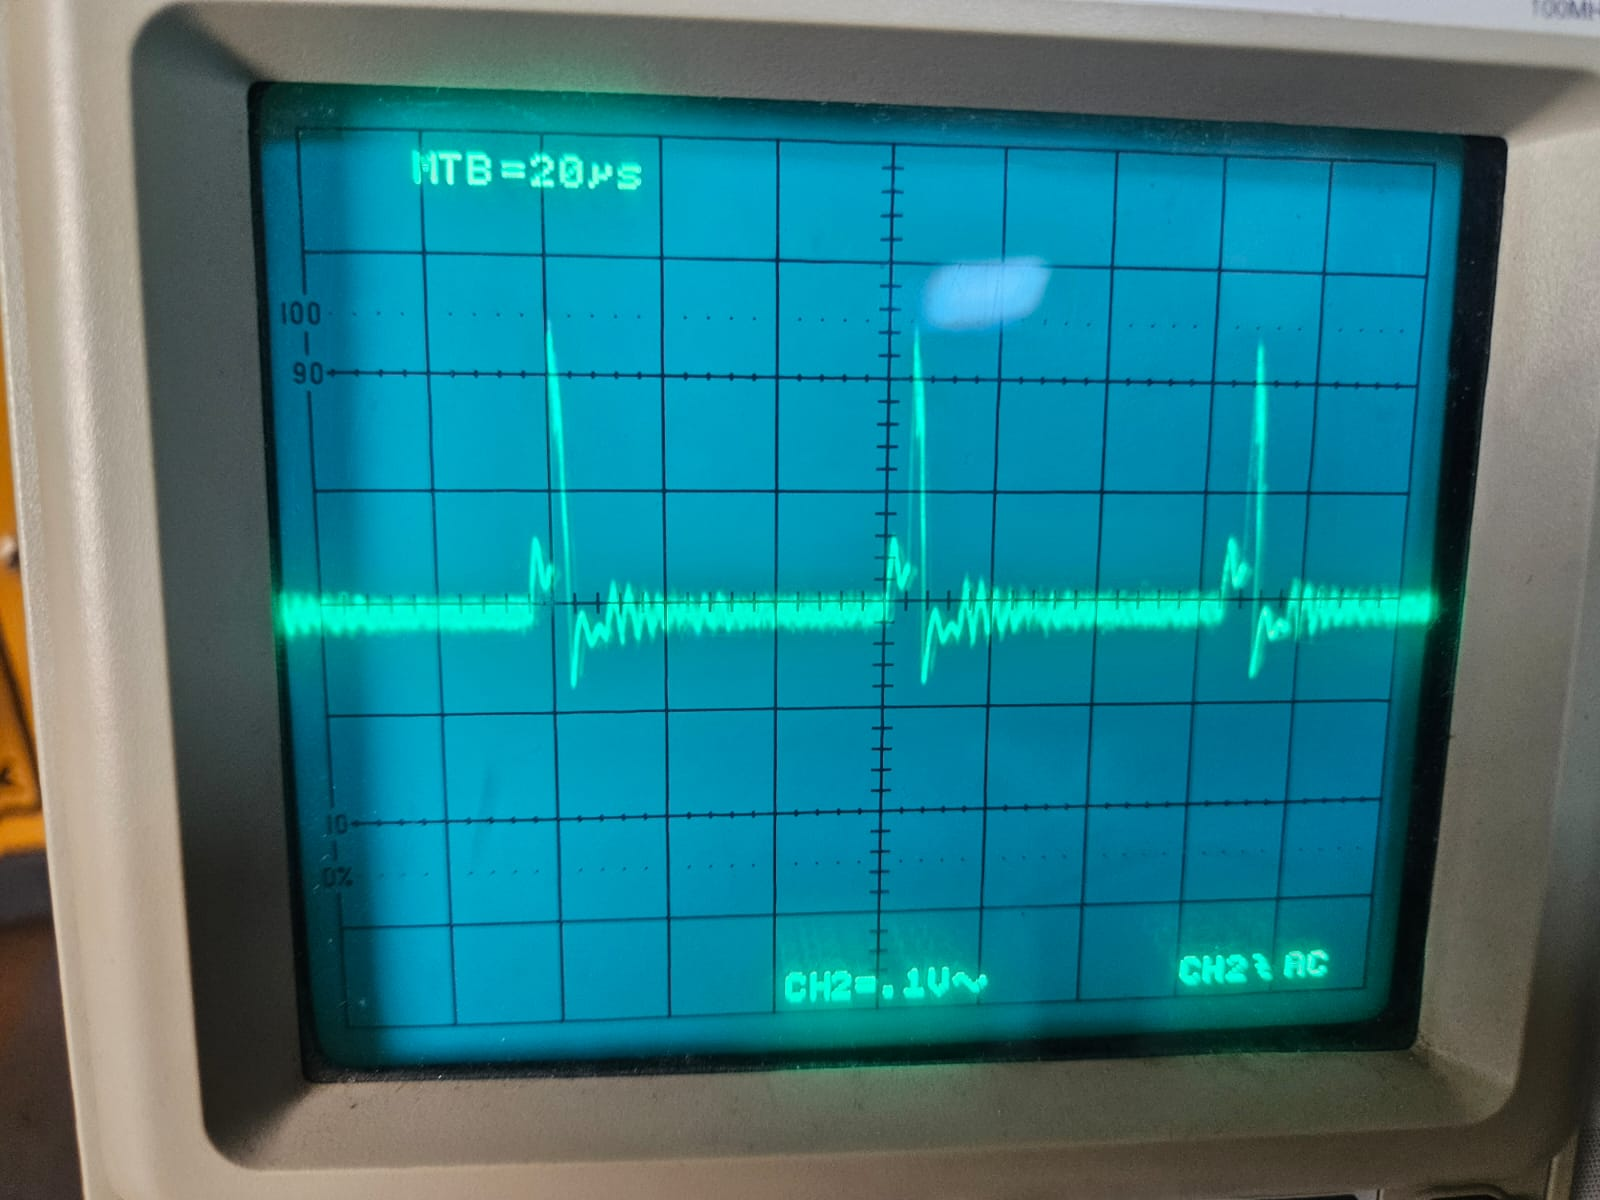
\includegraphics[width=1\linewidth]{Images/1.2}
		\caption{Fault 2}
		\vspace{0.1cm}
	\end{subfigure}
	
	\begin{subfigure}[t]{0.44\textwidth}
		\centering
		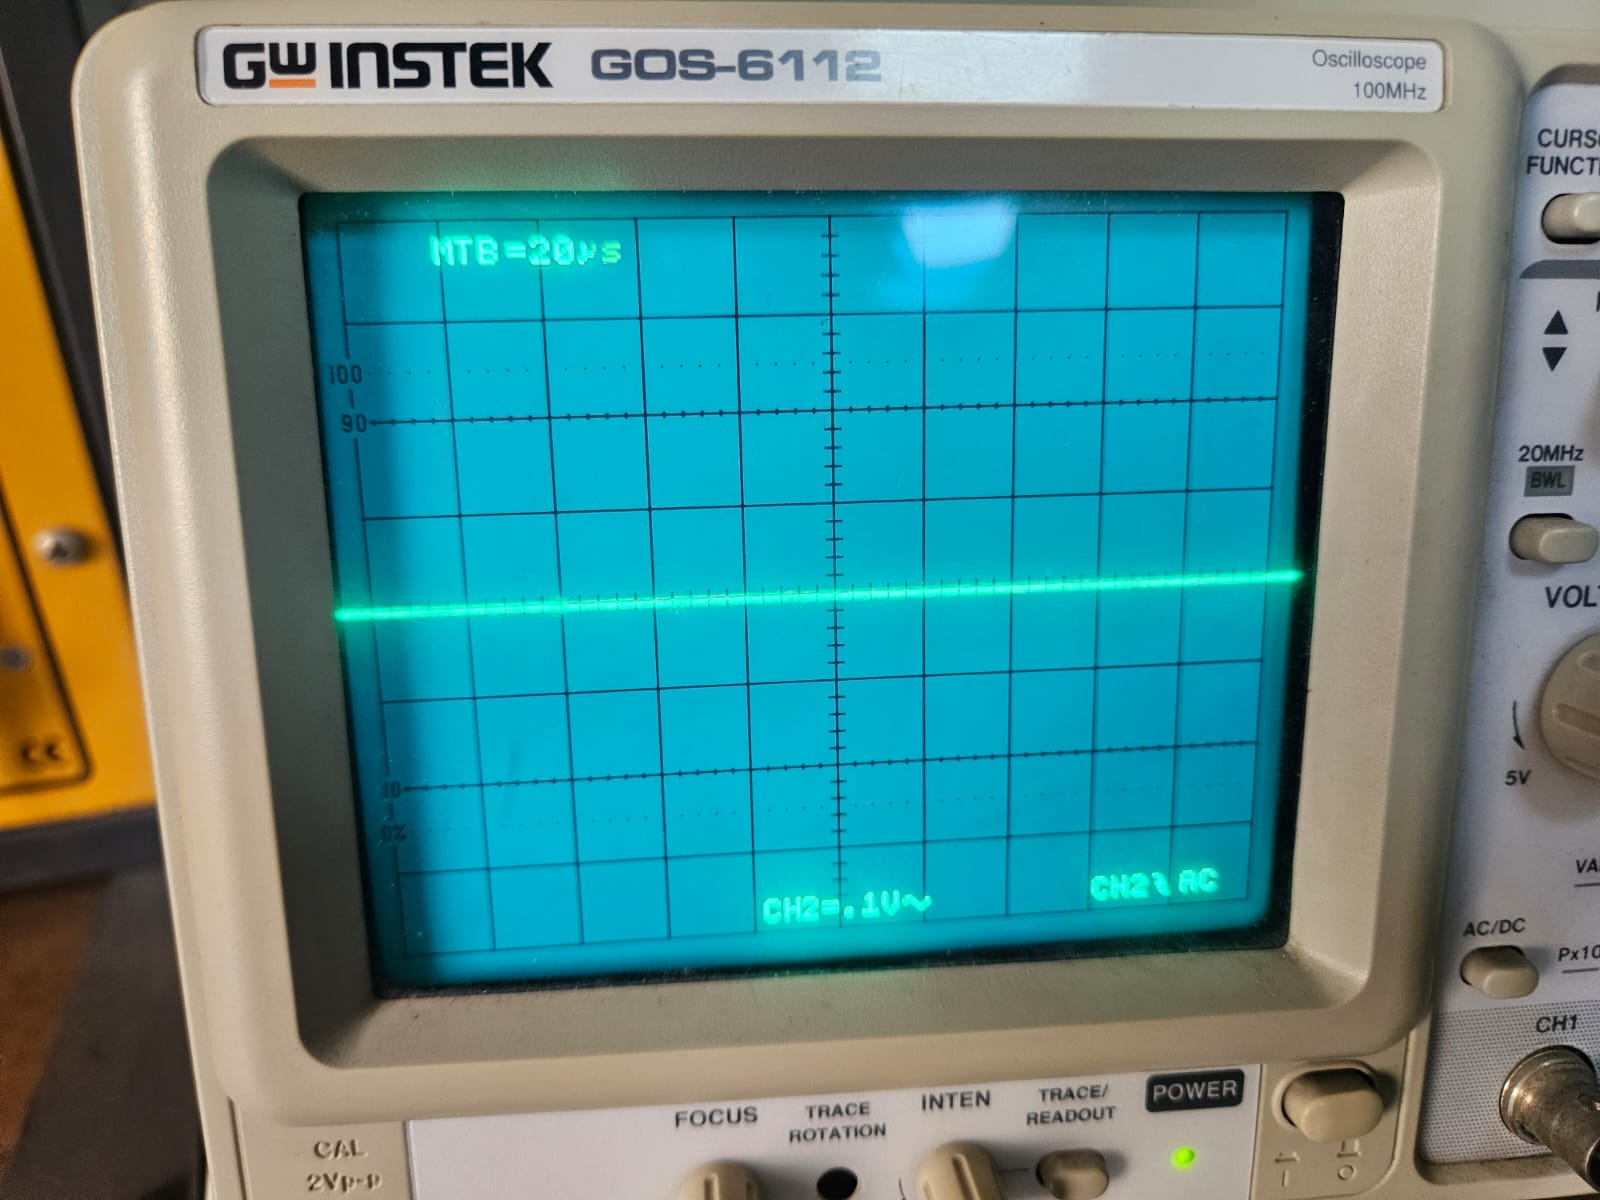
\includegraphics[width=1\linewidth]{Images/1.3}
		\caption{Fault 3}
		\vspace{0.1cm}
	\end{subfigure}
	\hfil
	\begin{subfigure}[t]{0.44\textwidth}
		\centering
		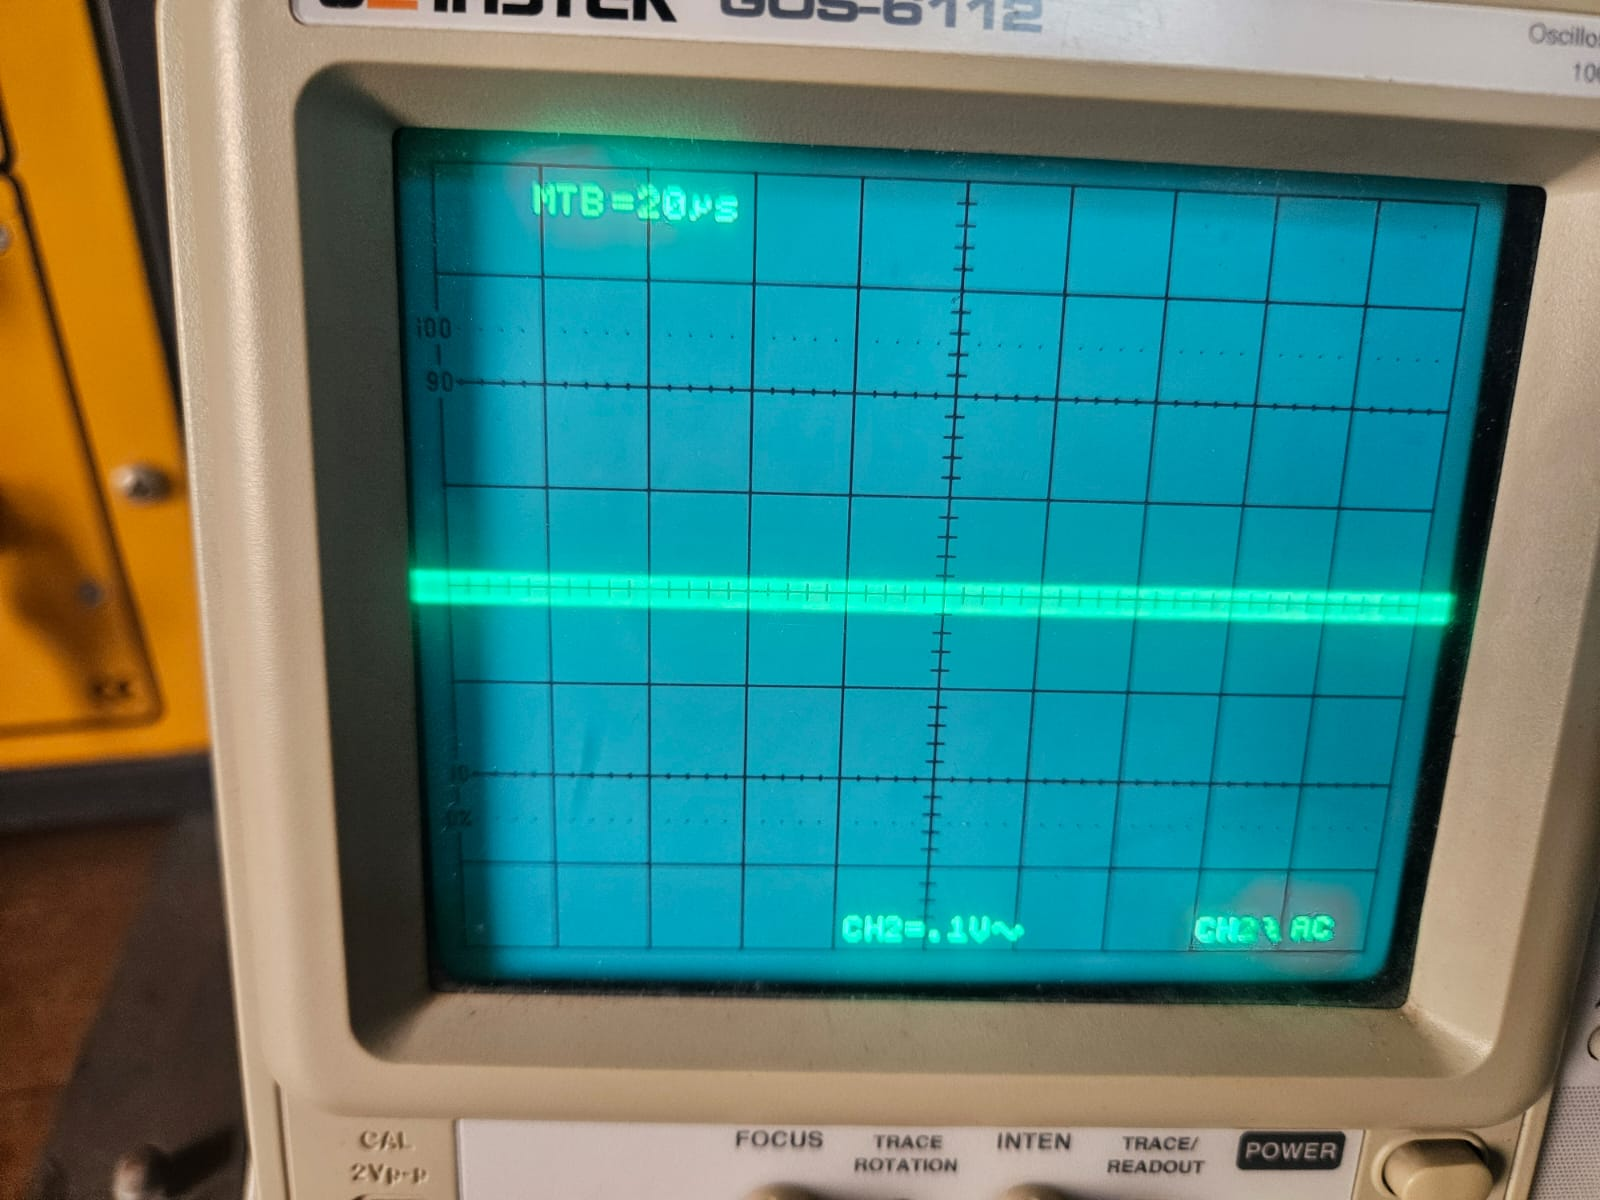
\includegraphics[width=1\linewidth]{Images/1.4}
		\caption{Fault 4}
		\vspace{0.1cm}
	\end{subfigure}
	
	
	\begin{subfigure}[t]{0.44\textwidth}
		\centering
		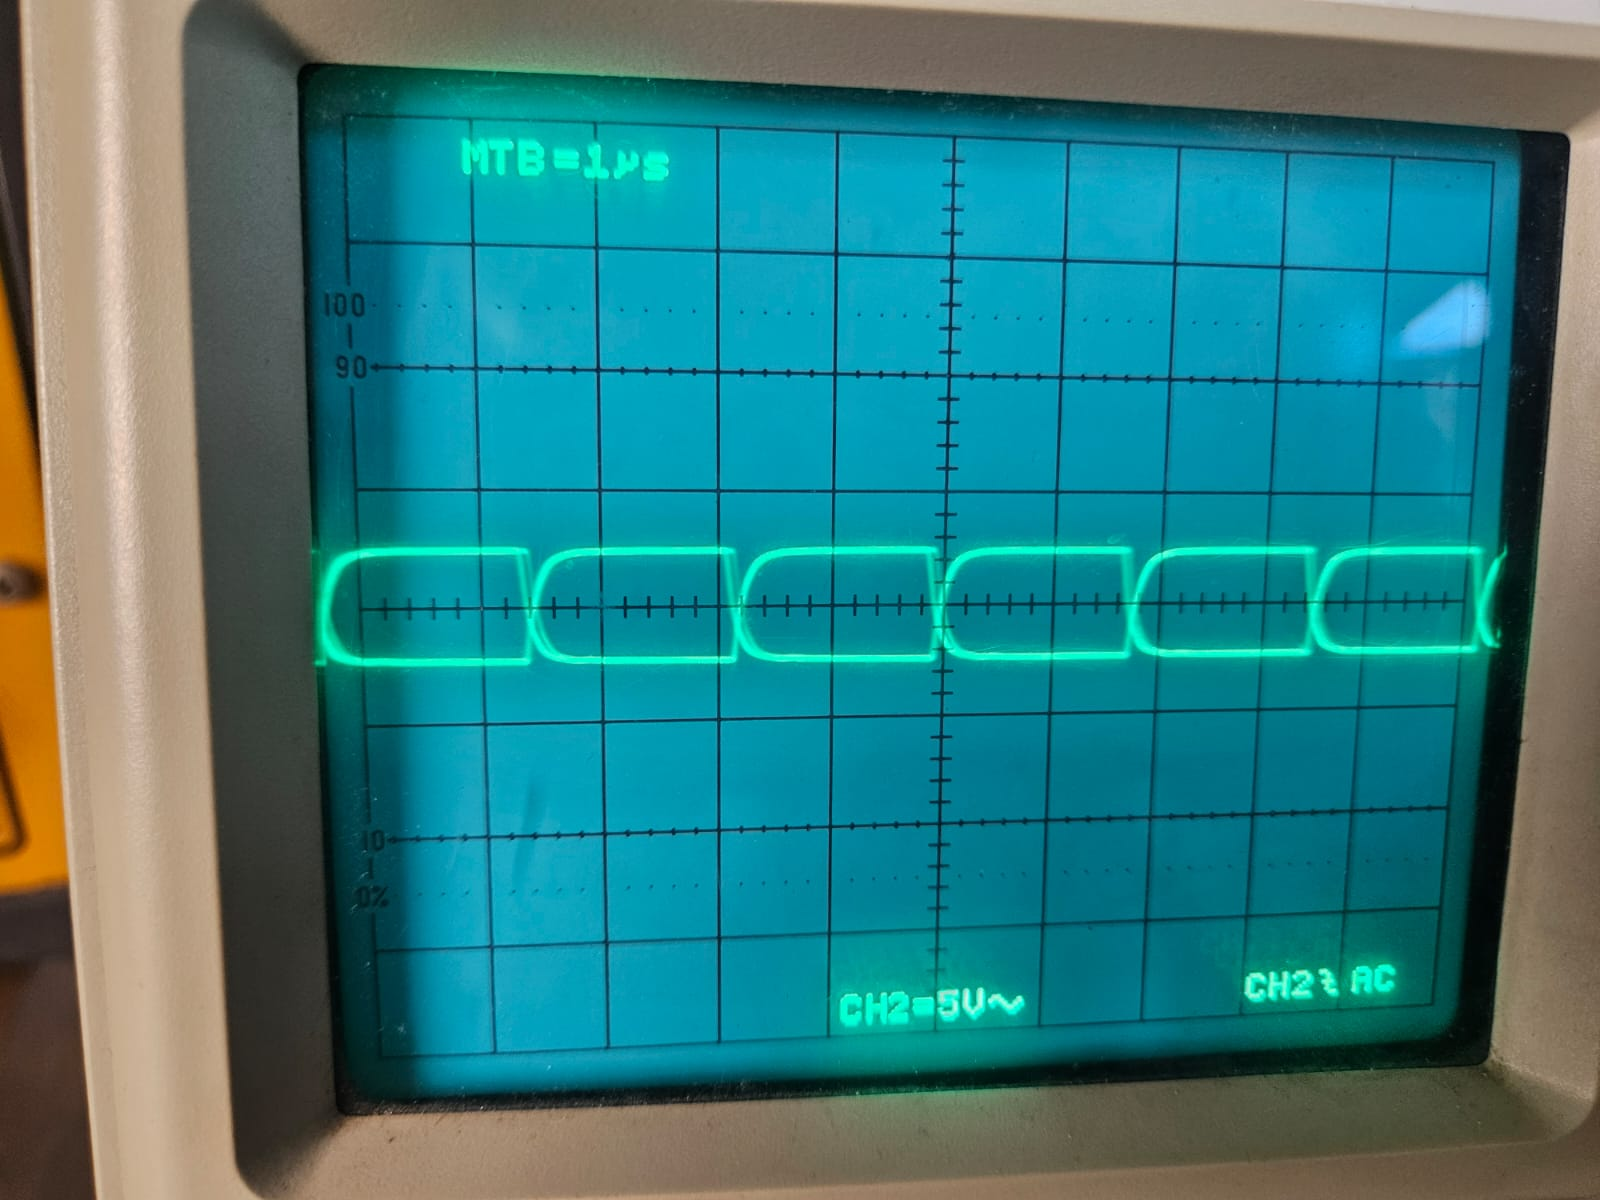
\includegraphics[width=1\linewidth]{Images/1.5}
		\caption{Fault 5}
		\vspace{0.1cm}
	\end{subfigure}
	\hfil
	\begin{subfigure}[t]{0.44\textwidth}
		\centering
		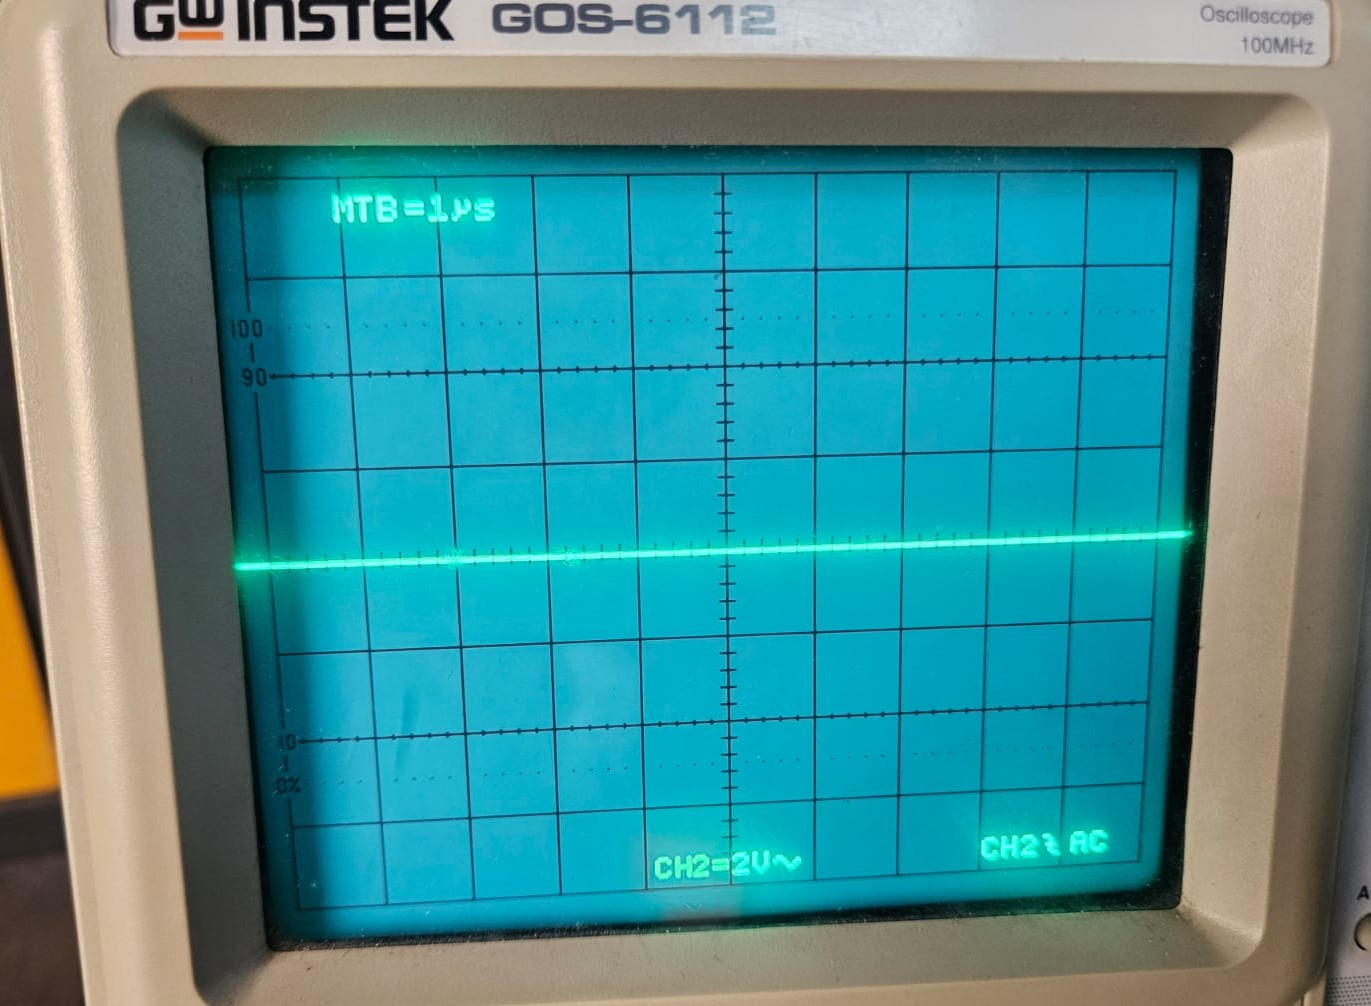
\includegraphics[width=1\linewidth]{Images/1.6}
		\caption{Fault 6}
		\vspace{0.1cm}
	\end{subfigure}
	
	\begin{subfigure}[t]{0.44\textwidth}
		\centering
		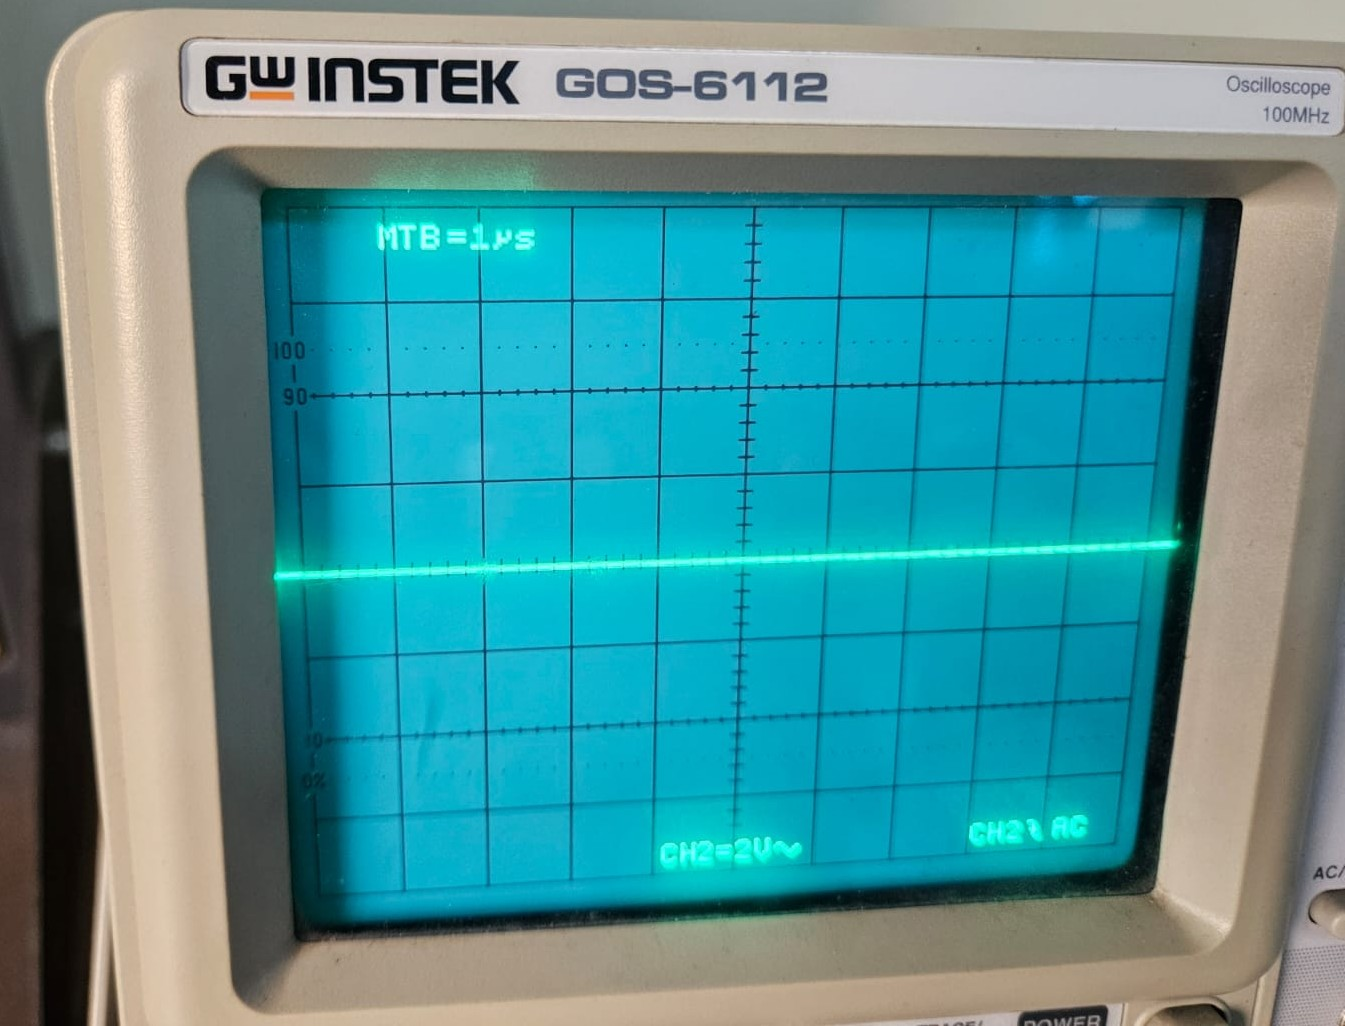
\includegraphics[width=1\linewidth]{Images/1.7}
		\caption{Fault 7}
		\vspace{0.1cm}
	\end{subfigure}
	\hfil
	\begin{subfigure}[t]{0.44\textwidth}
		\centering
		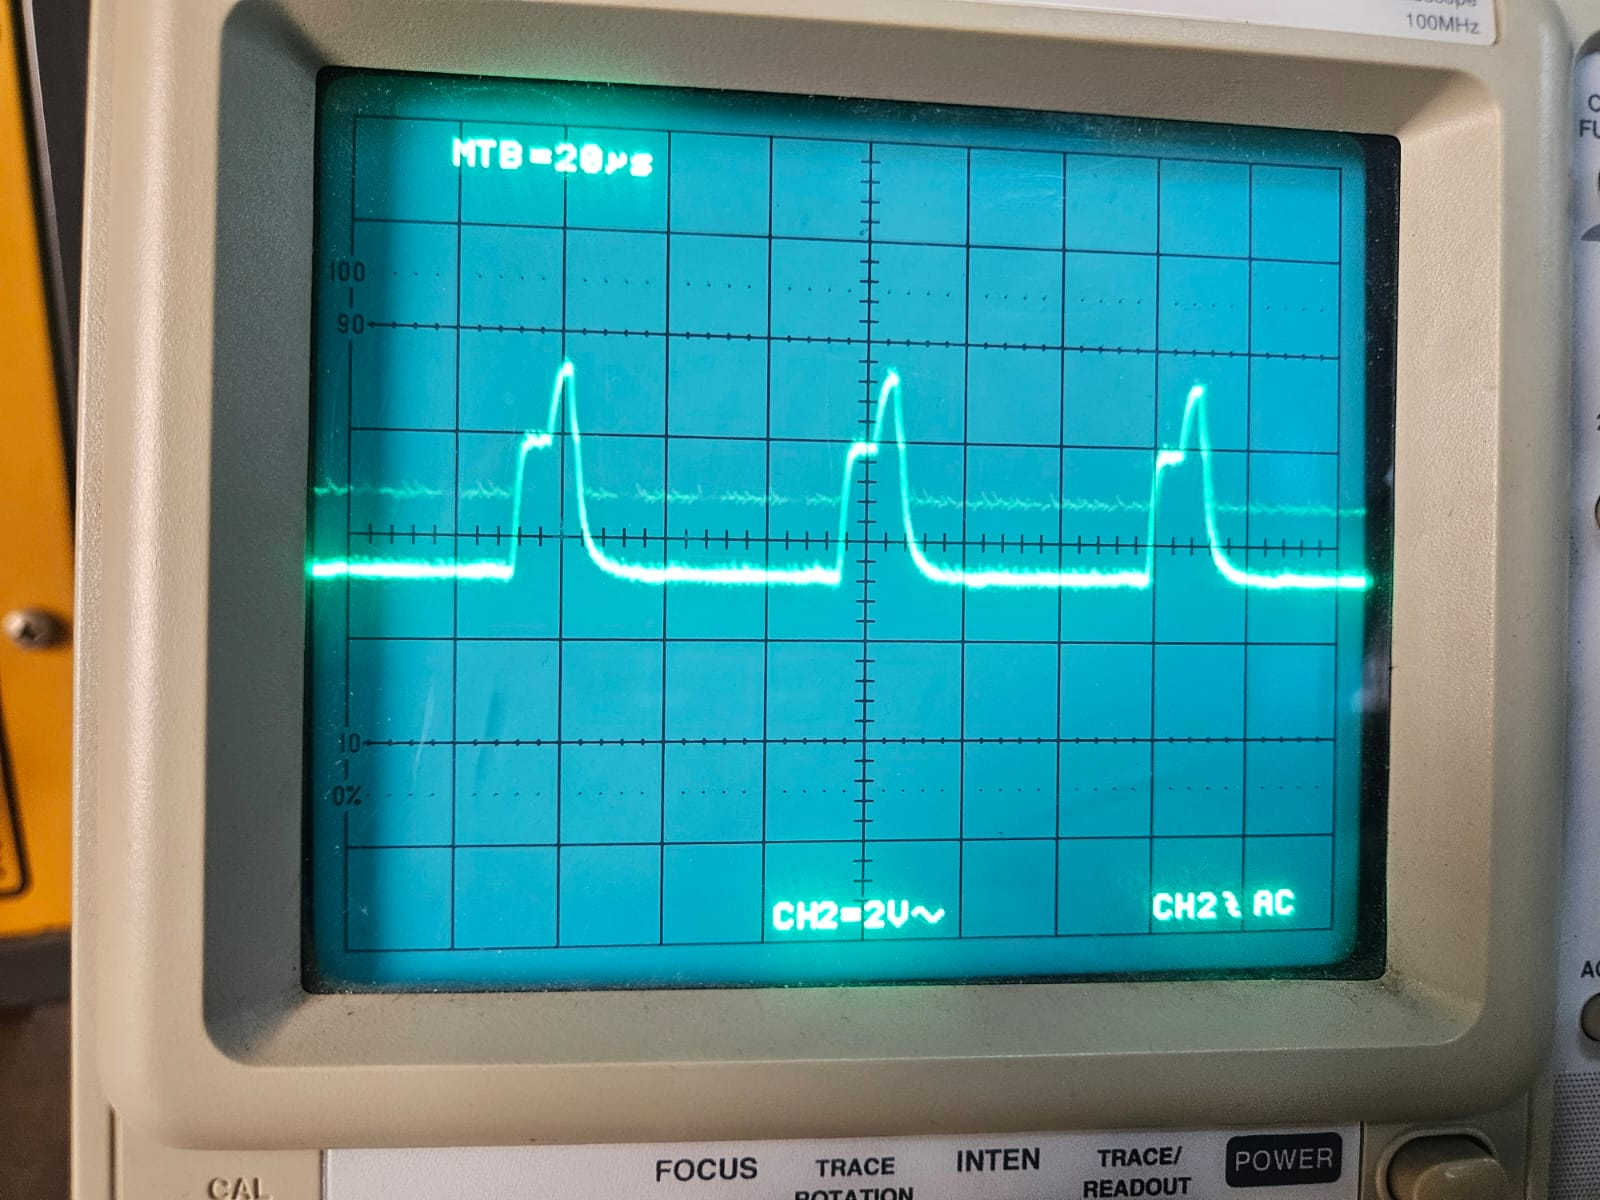
\includegraphics[width=1\linewidth]{Images/1.8}
		\caption{Fault 8}
		\vspace{0.1cm}
	\end{subfigure}
	%%%%%%%%%%%%
\end{figure}




%%%%%%%%%%%%%%%%%%%%%%%%%%%%%%%%%%%%%%%%%%%%%
\begin{figure}[H]
	\centering
	\begin{subfigure}[t]{0.44\textwidth}
		\centering
		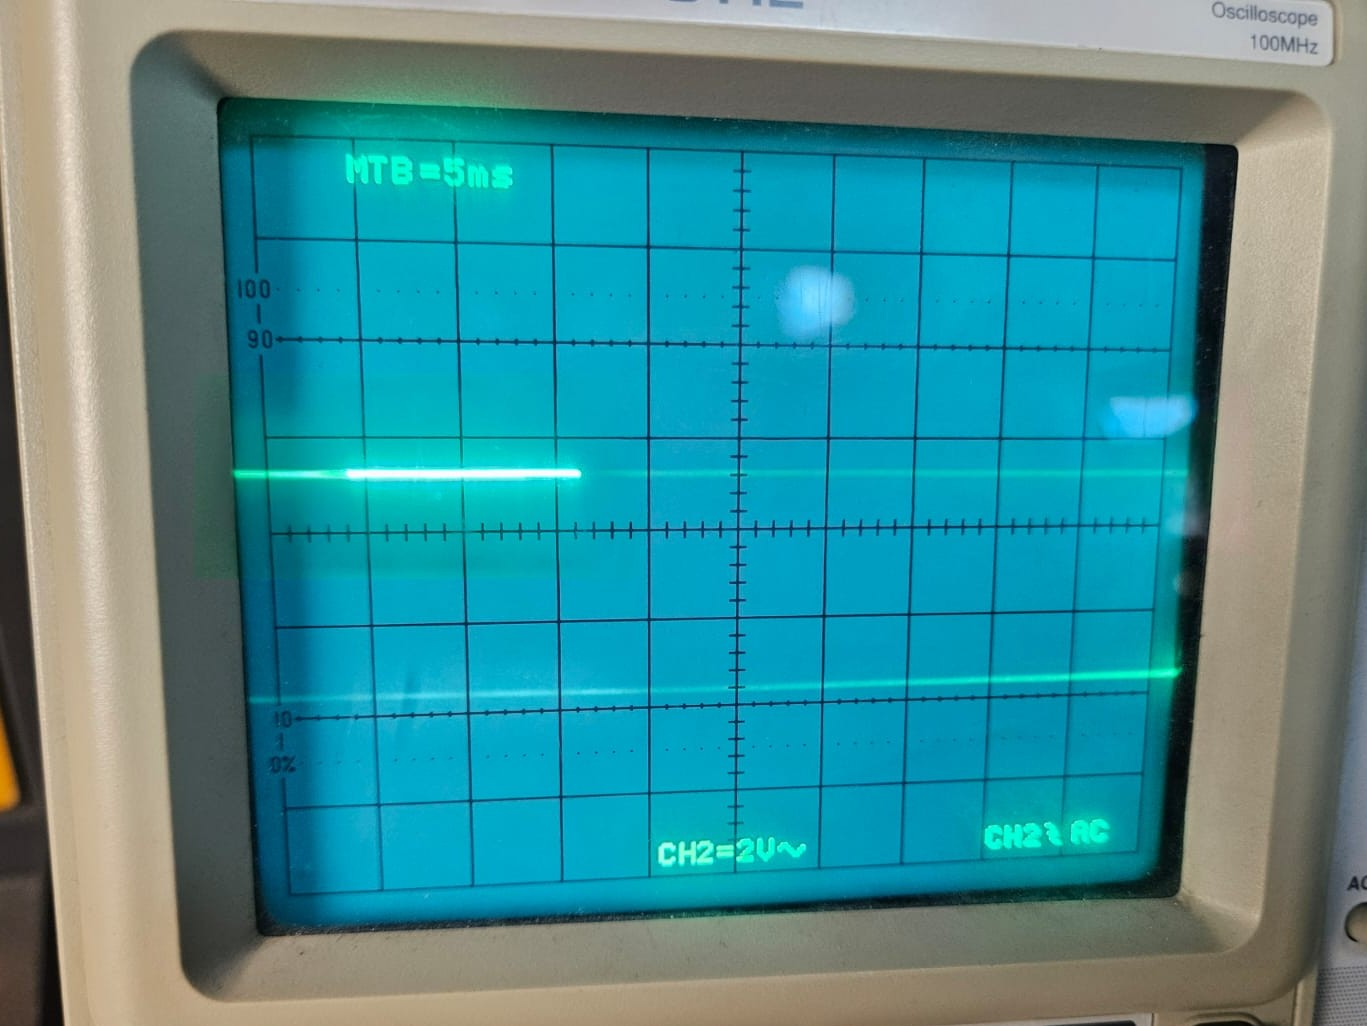
\includegraphics[width=1\linewidth]{Images/1.9}
		\caption{Fault 9}
		\vspace{0.1cm}
	\end{subfigure}
	\hfil
	\begin{subfigure}[t]{0.44\textwidth}
		\centering
		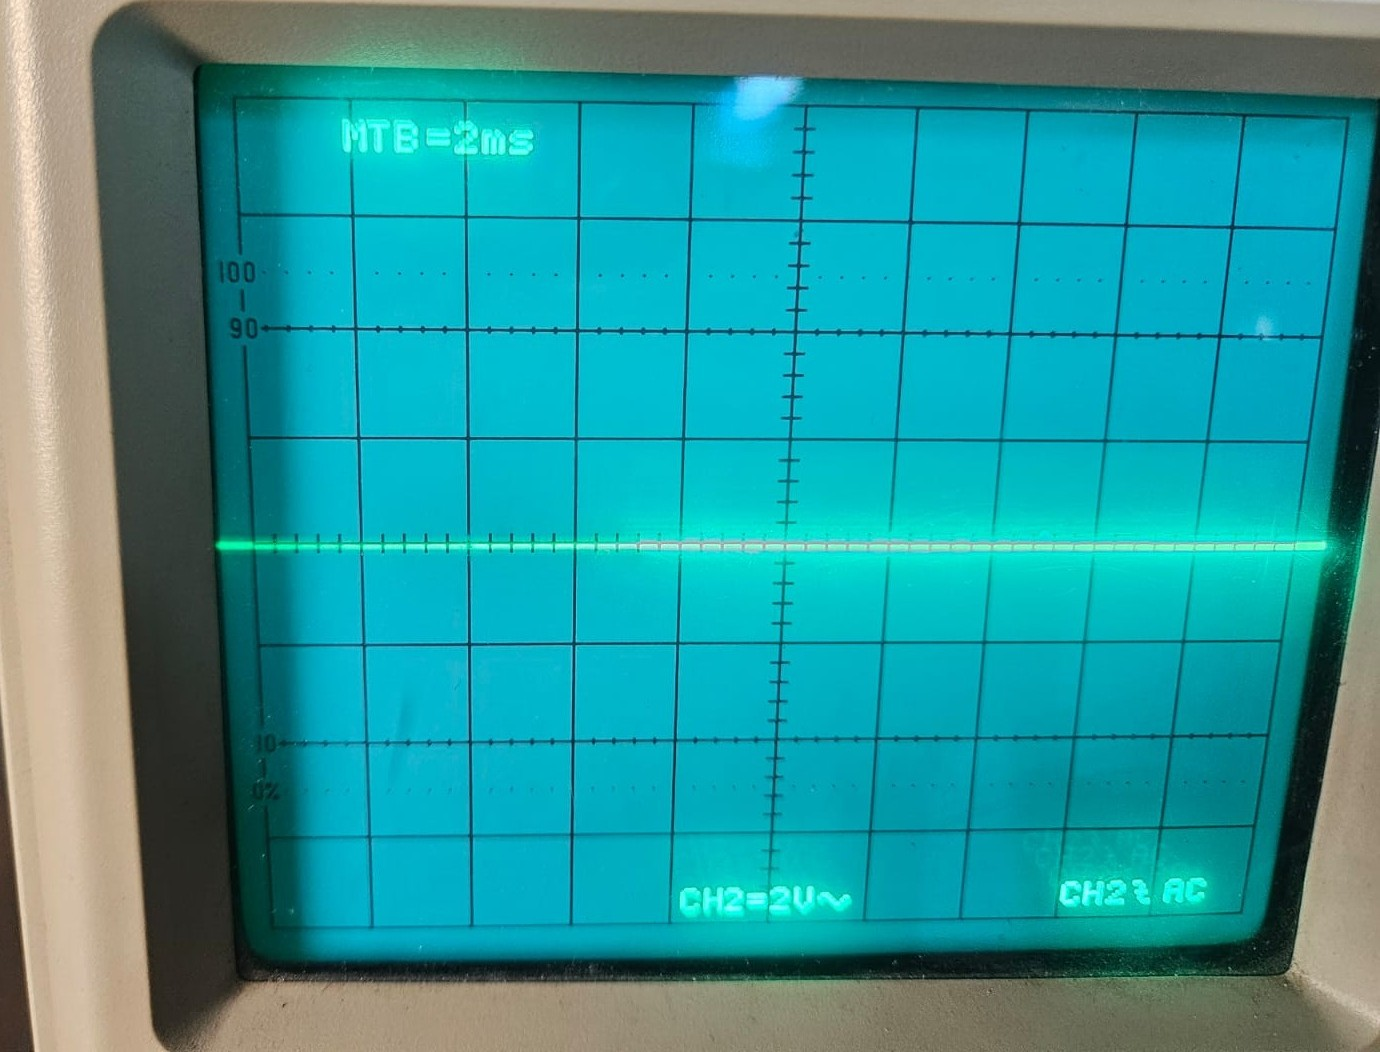
\includegraphics[width=1\linewidth]{Images/1.10}
		\caption{Fault 10}
		\vspace{0.1cm}
	\end{subfigure}
	
	\begin{subfigure}[t]{0.44\textwidth}
		\centering
		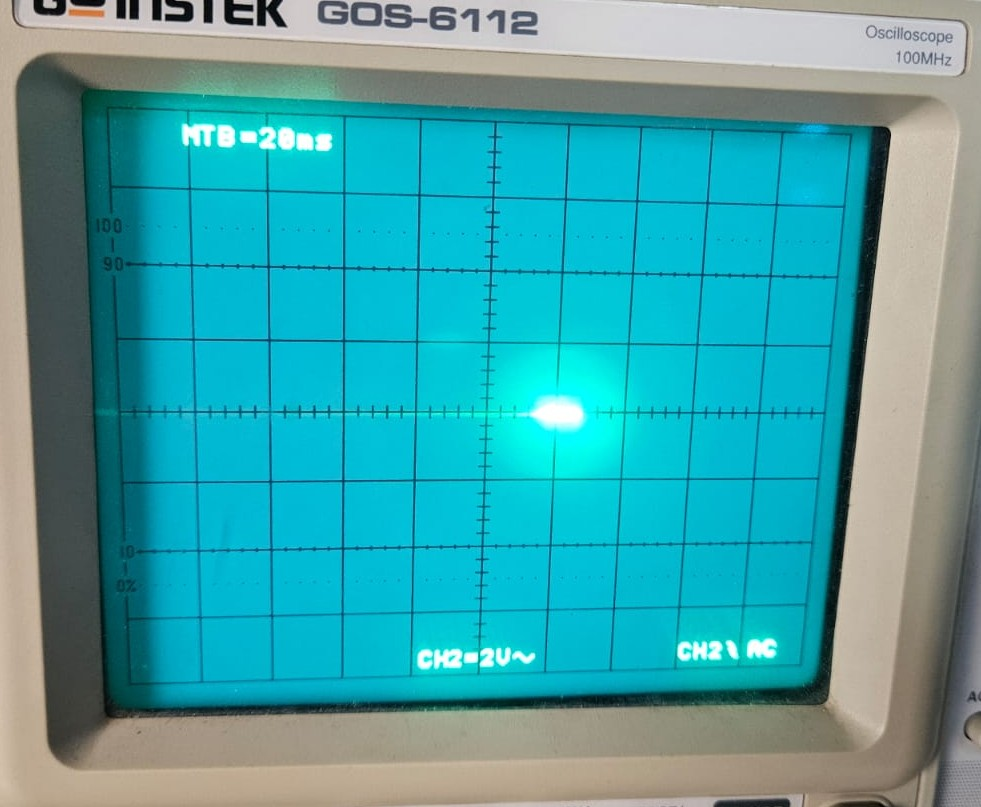
\includegraphics[width=1\linewidth]{Images/1.11}
		\caption{Fault 11}
		\vspace{0.1cm}
	\end{subfigure}
	\hfil
	\begin{subfigure}[t]{0.44\textwidth}
		\centering
		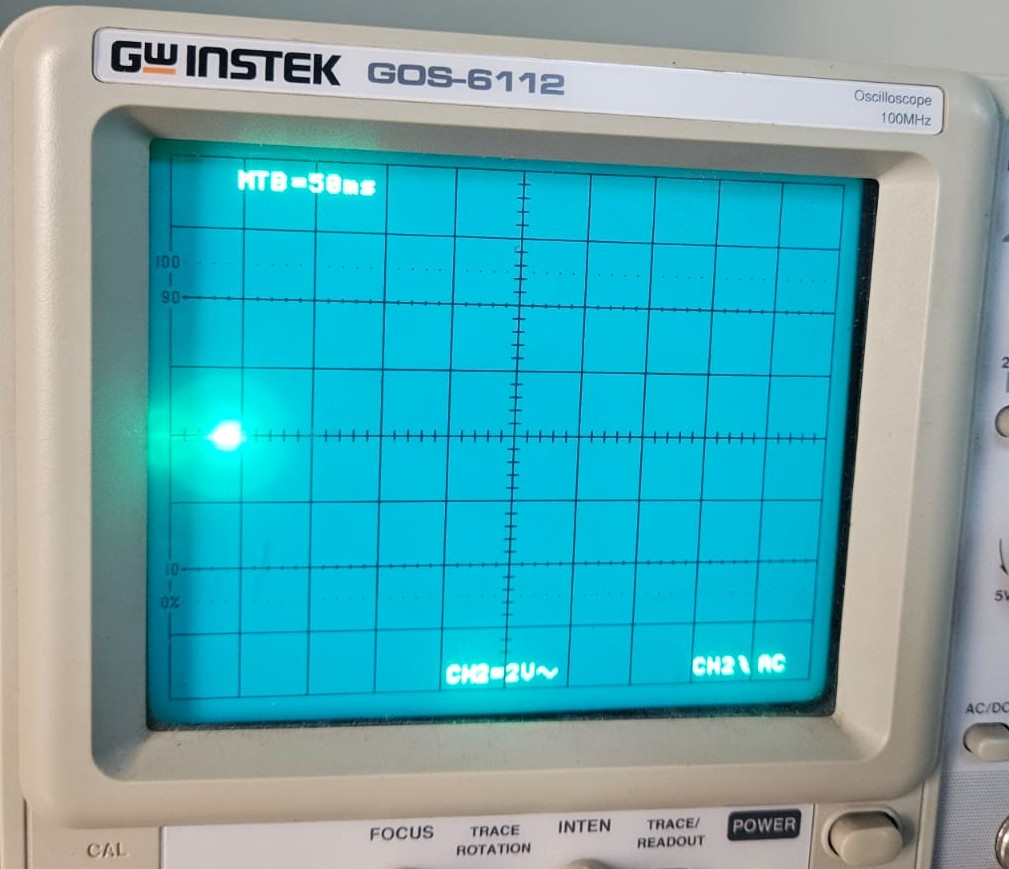
\includegraphics[width=1\linewidth]{Images/1.12}
		\caption{Fault 12}
		\vspace{0.1cm}
	\end{subfigure}
	
	%%%%%%%%%%%
	\begin{subfigure}[t]{0.44\textwidth}
		\centering
		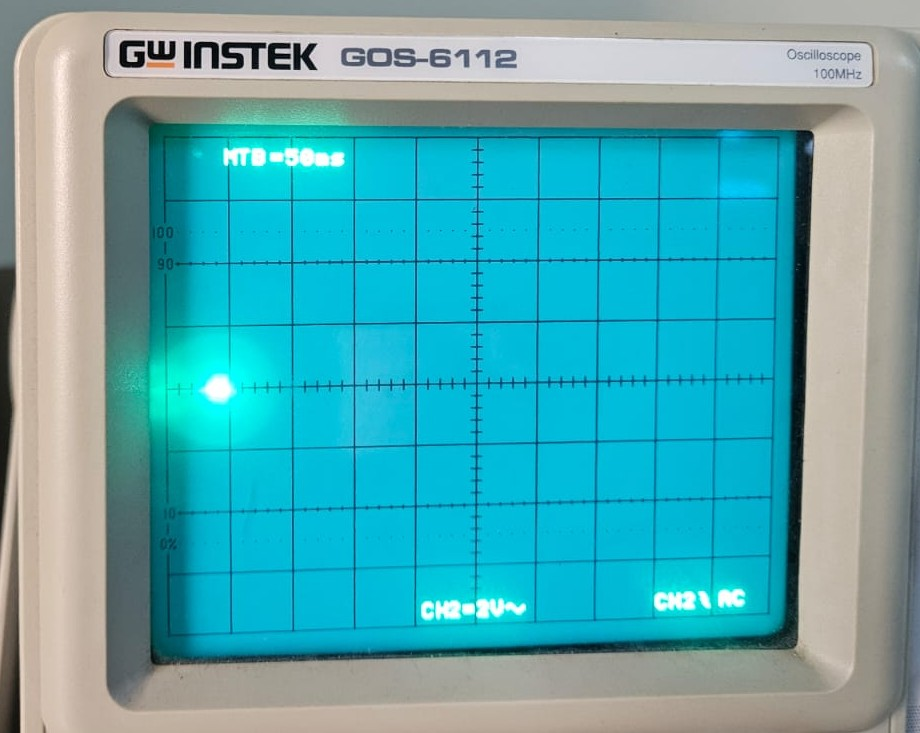
\includegraphics[width=1\linewidth]{Images/1.13}
		\caption{Fault 13}
		\vspace{0.1cm}
	\end{subfigure}
	\hfil
	\begin{subfigure}[t]{0.44\textwidth}
		\centering
		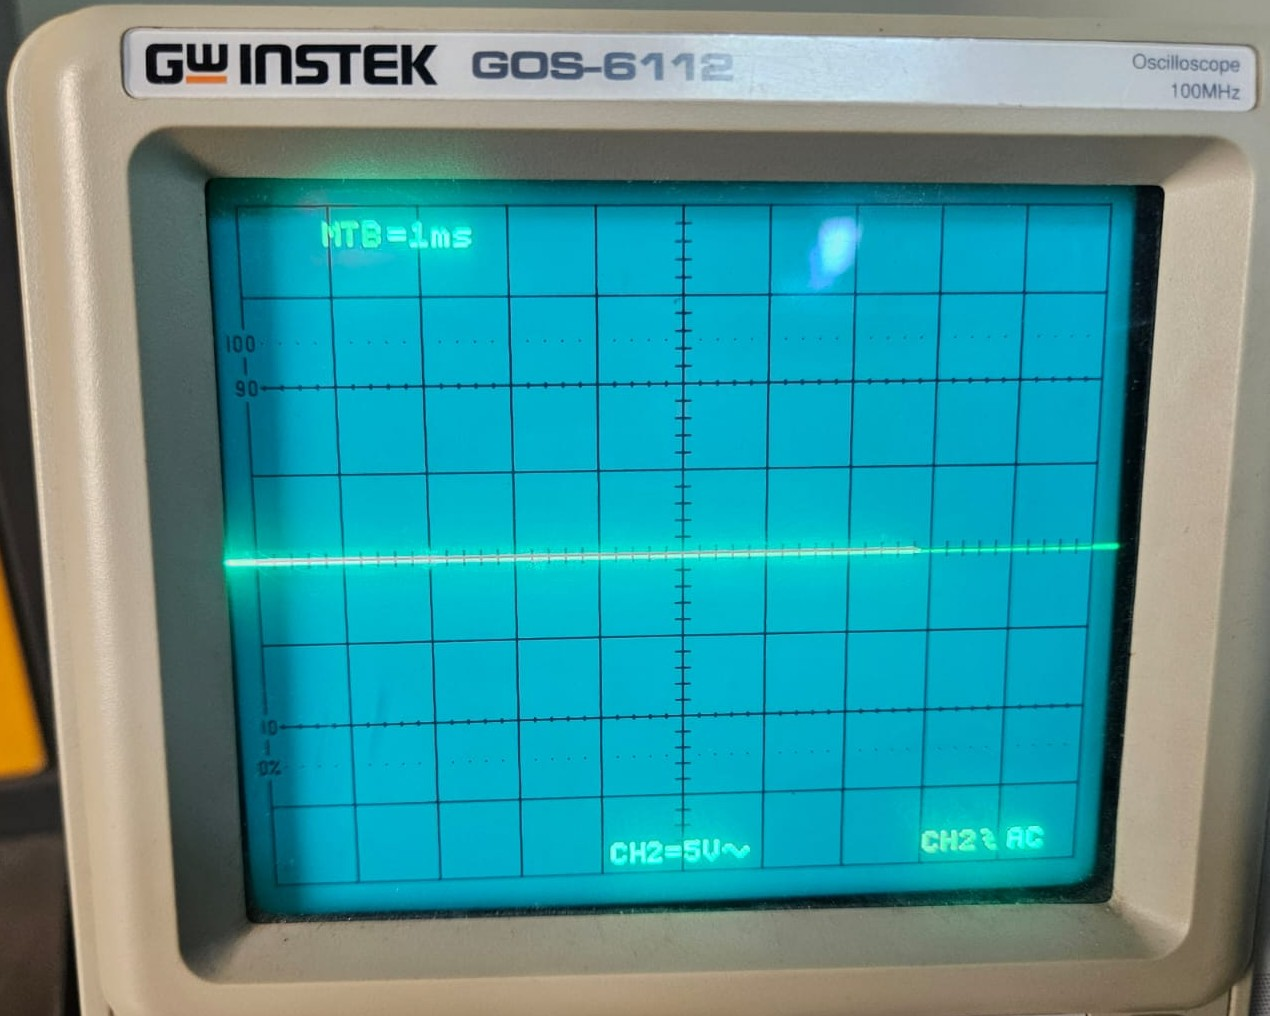
\includegraphics[width=1\linewidth]{Images/1.14}
		\caption{Fault 14}
		\vspace{0.1cm}
	\end{subfigure}
	
	\begin{subfigure}[t]{0.44\textwidth}
		\centering
		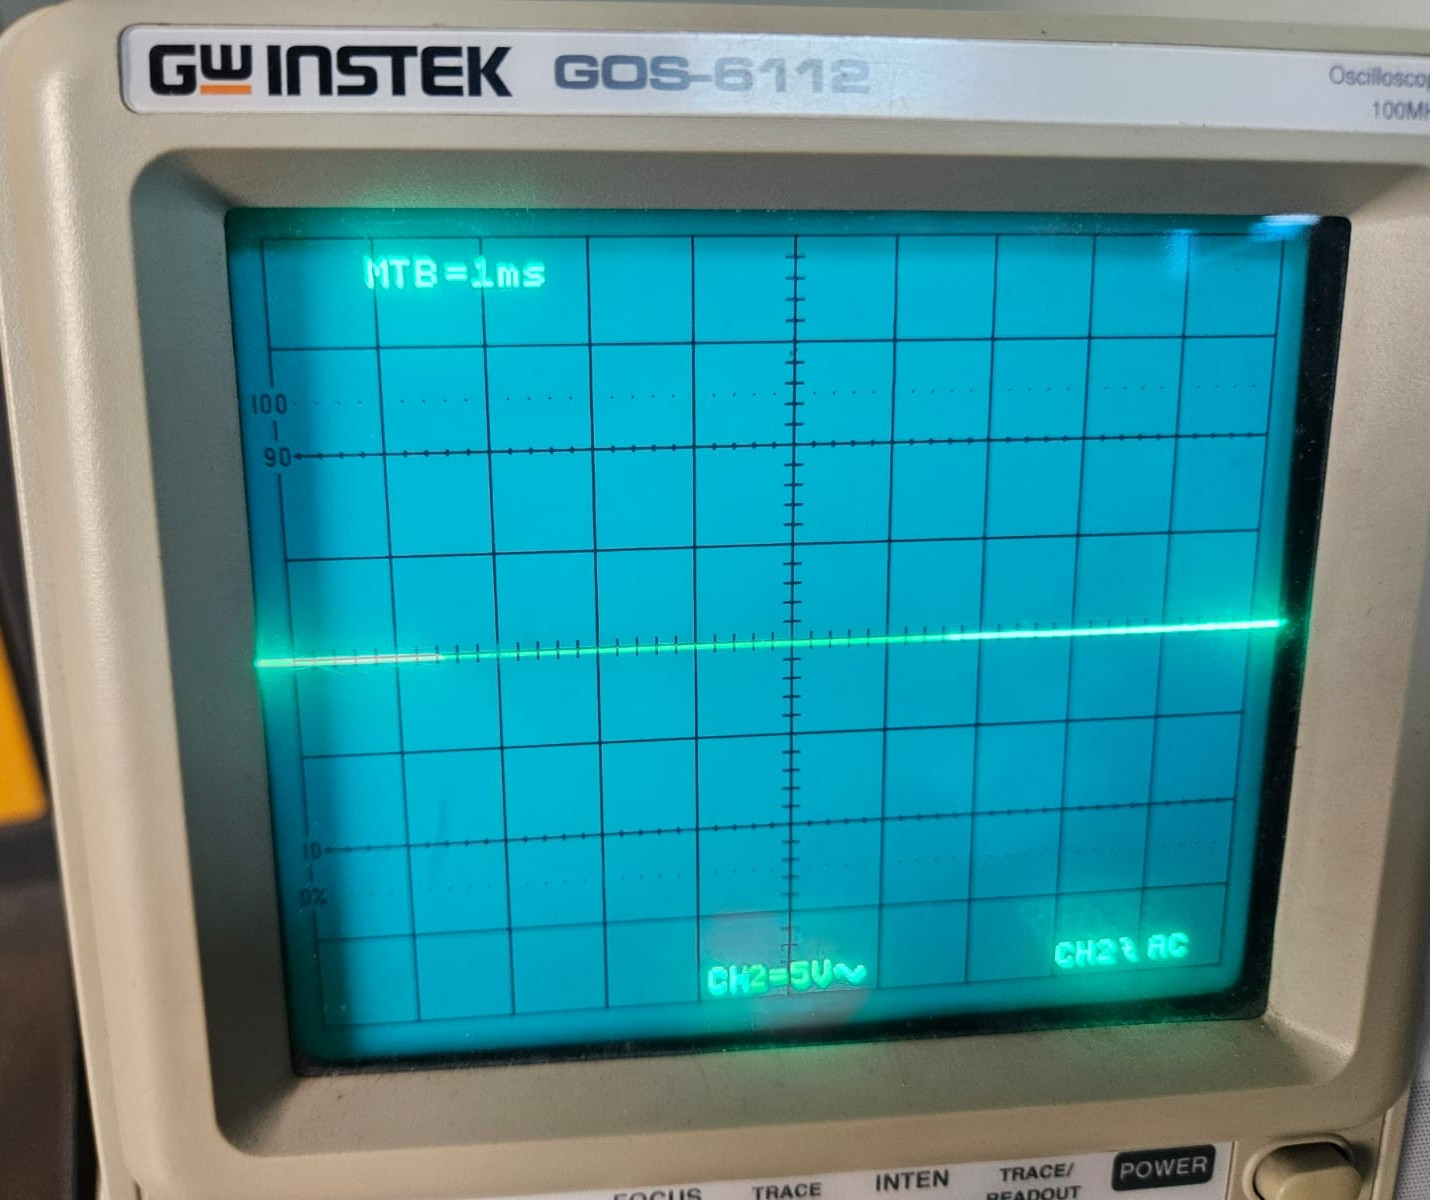
\includegraphics[width=1\linewidth]{Images/1.15}
		\caption{Fault 15}
		\vspace{0.1cm}
	\end{subfigure}
	\hfil
	\begin{subfigure}[t]{0.44\textwidth}
		\centering
		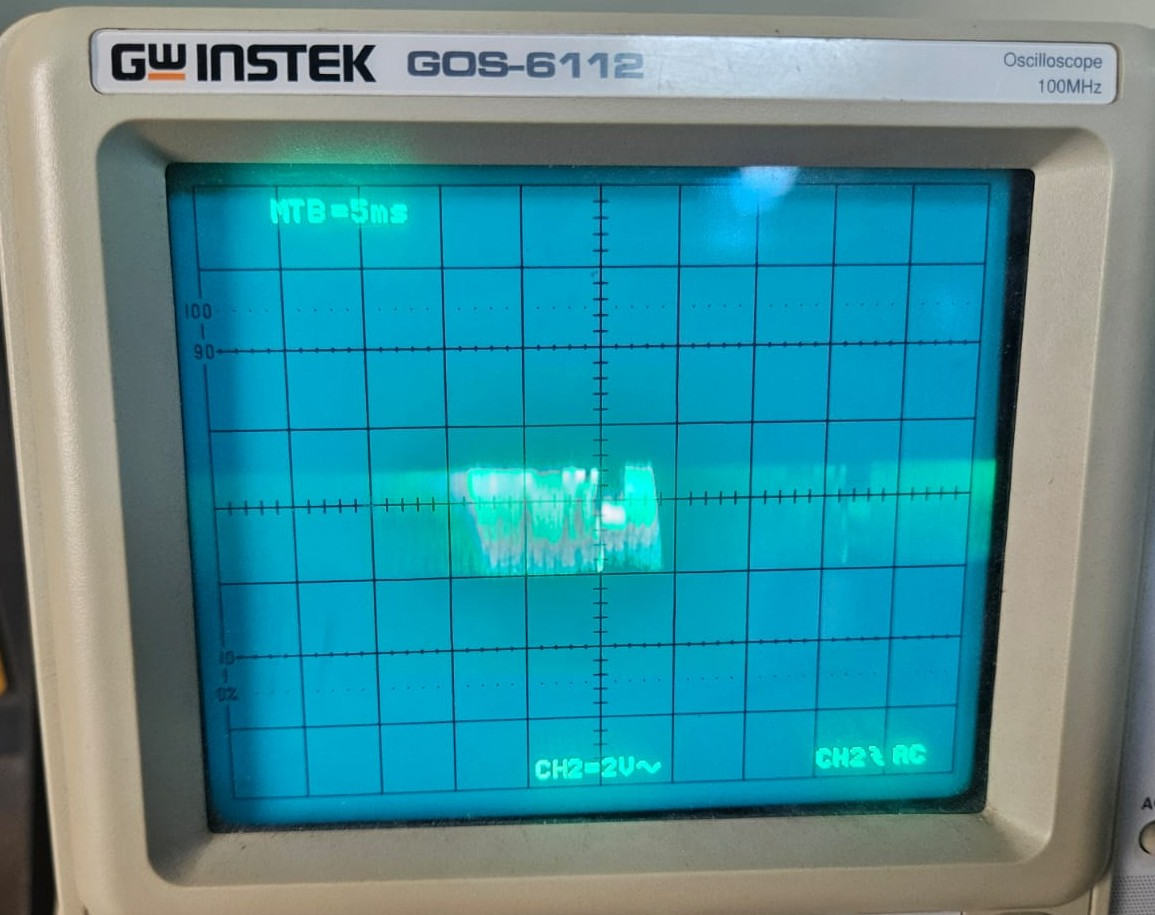
\includegraphics[width=1\linewidth]{Images/1.16}
		\caption{Fault 16}
		\vspace{0.1cm}
	\end{subfigure}
	%%%%%%%%%%
\end{figure}


\begin{figure}[H]
	\centering
	
	\begin{subfigure}[t]{0.44\textwidth}
		\centering
		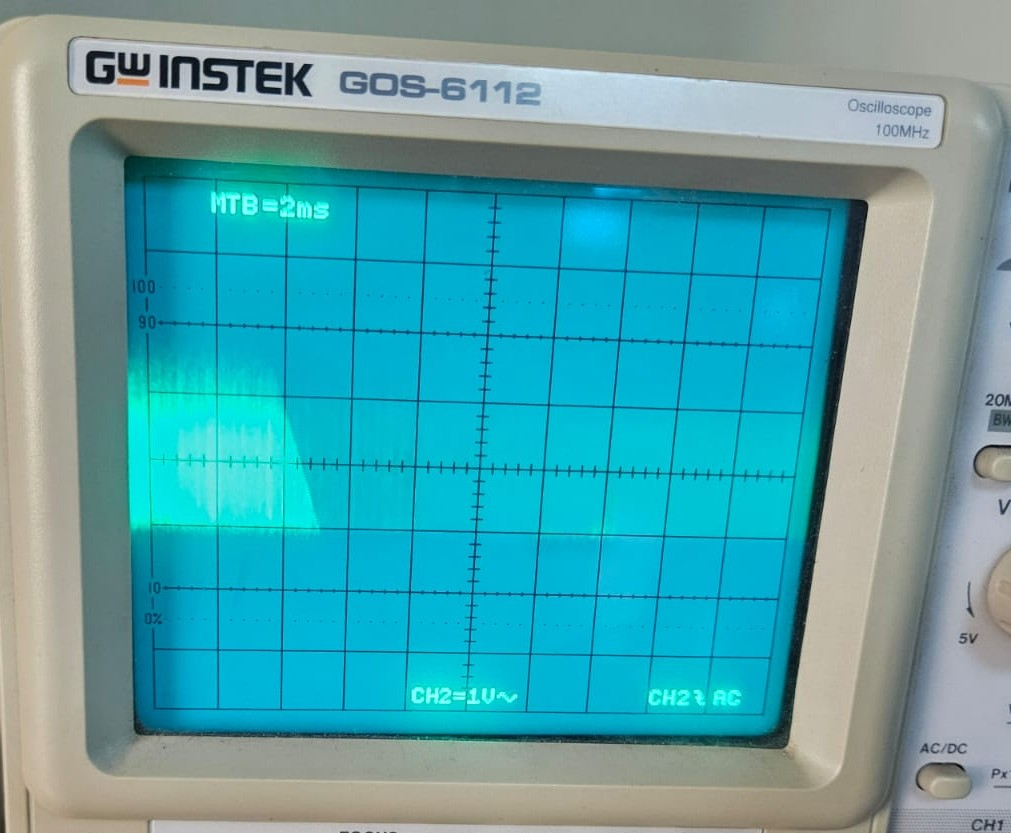
\includegraphics[width=1\linewidth]{Images/1.17}
		\caption{Fault 17}
		\vspace{0.1cm}
	\end{subfigure}
	\hfil
	\begin{subfigure}[t]{0.44\textwidth}
		\centering
		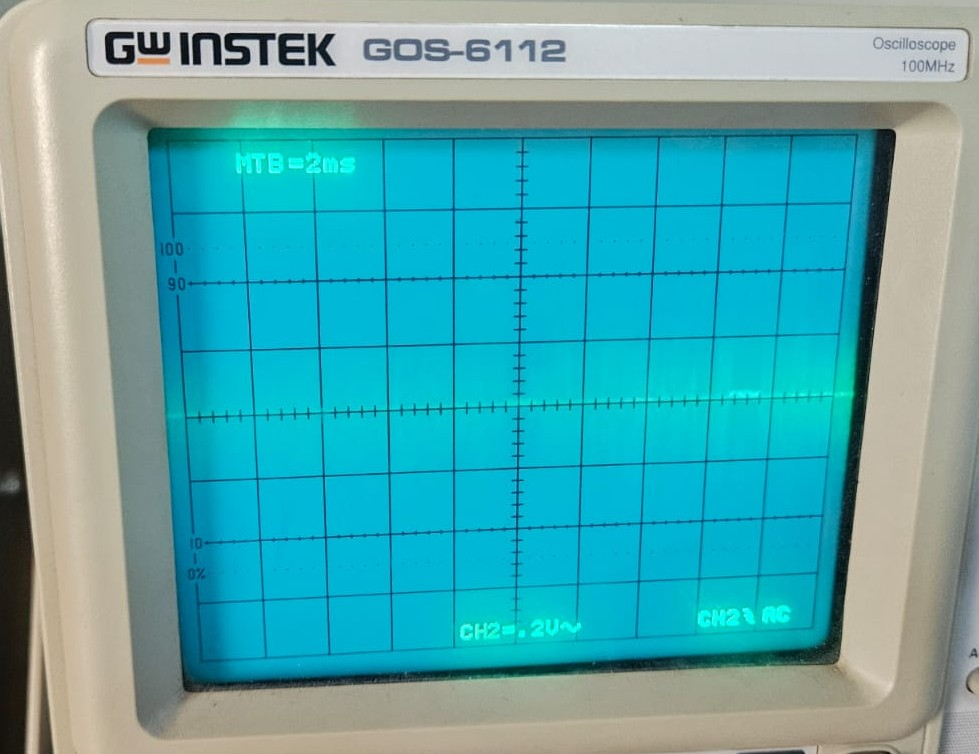
\includegraphics[width=1\linewidth]{Images/1.18}
		\caption{Fault 18}
		\vspace{0.1cm}
	\end{subfigure}
	
	\begin{subfigure}[t]{0.44\textwidth}
		\centering
		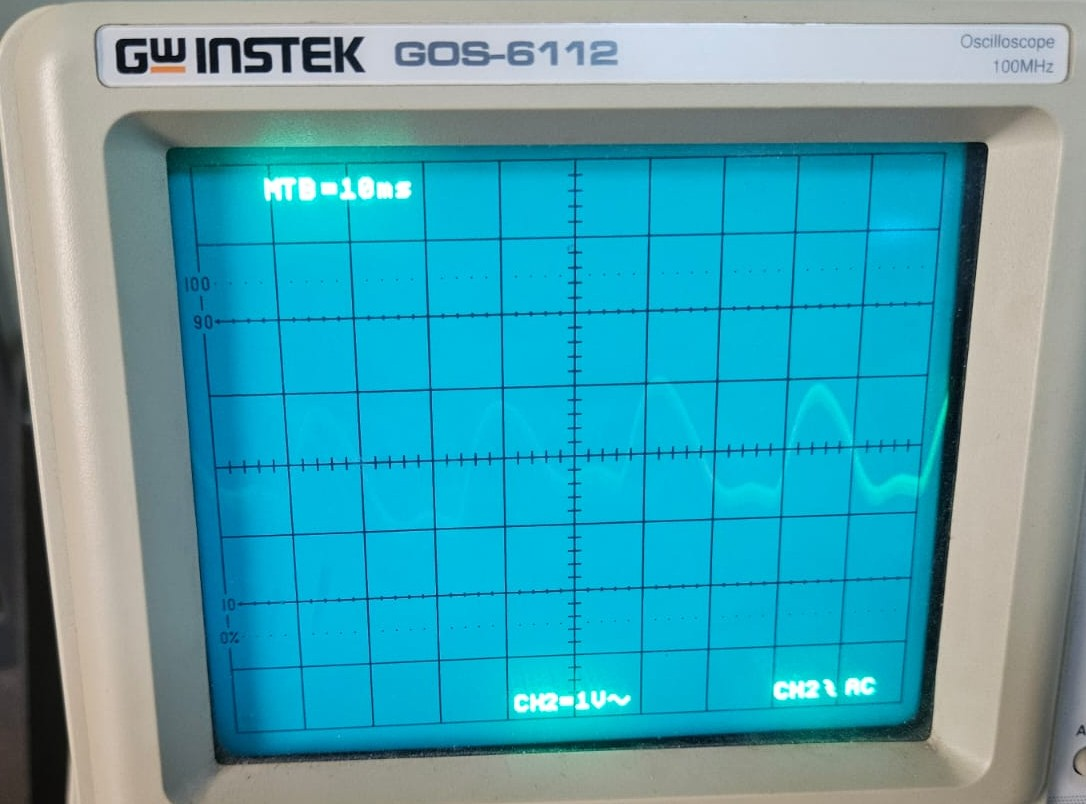
\includegraphics[width=1\linewidth]{Images/1.19}
		\caption{Fault 19}
		\vspace{0.1cm}
	\end{subfigure}
	\hfil
	\begin{subfigure}[t]{0.44\textwidth}
		\centering
		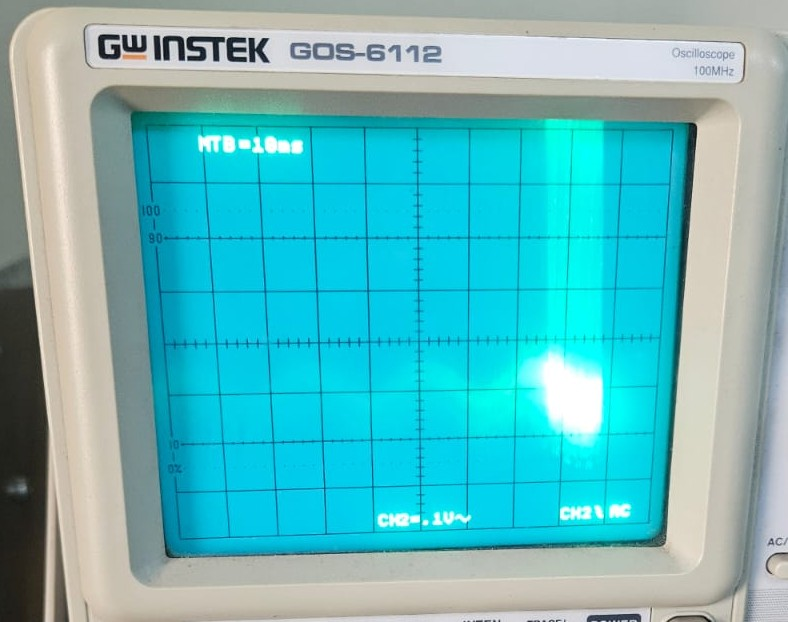
\includegraphics[width=1\linewidth]{Images/1.20}
		\caption{Fault 20}
		\vspace{0.1cm}
	\end{subfigure}
	
	
\end{figure}


	\section{Discussion}
	
	
In this laboratory experiment, the analysis of fault locations and observations was done using two primary trainers: an LCD/LED TV Trainer (KVT-05A/B Trainer Kit) and a DL 2402 Color TV Trainer.

For the LED TV fault analysis, several types of faults were investigated, including those related to the IR remote, keyboard, audio, video, and display. By switching off specific DIP switches, each of these faults was successfully analyzed.

Regarding the cathode ray TV fault analysis, a total of 20 faults were intended to be analyzed; however, some of these did not function in accordance with the laboratory manual. For certain faults, the TV was required to be restarted to ensure proper operation. Simultaneously, the oscilloscope output was observed to understand the nature of each fault.

\end{document}